\documentclass[10pt]{amsart}
\usepackage[a4paper,margin=23mm]{geometry}
\usepackage{amsmath,amssymb,amsthm,mathtools,hyperref,graphicx,xspace,letltxmacro,xpatch}
\usepackage[english]{babel}
\newtheorem{theo}{Theorem}[section]
\newtheorem{lemm}[theo]{Lemma}\newtheorem{prop}[theo]{Proposition}\newtheorem{coro}[theo]{Corollary}\newtheorem{conj}[theo]{Conjecture}
\theoremstyle{definition}\newtheorem{defi}[theo]{Definition}\newtheorem{rema}[theo]{Remark}\newtheorem{exam}[theo]{Example}\newtheorem{exem}[theo]{Example}\newtheorem{nota}[theo]{Notation}
\newcommand{\ie}{i.e.}\newcommand{\eg}{e.g.}\newcommand{\resp}{resp.}\newcommand{\skpt}{\par\smallskip\noindent}
\emergencystretch=3em\pagestyle{plain}

\usepackage{dsfont}



\newcommand{\psiw}{\psi_{\mathtt w}}

\newcommand{\ttw}{\mathtt{w}}
\newcommand{\ttW}{\mathtt{W}}

\newcommand{\bbE}{\mathbb{E}}
\newcommand{\bbZ}{\mathbb{Z}}
\newcommand{\bbN}{\mathbb{N}}
\newcommand{\bbC}{\mathbb{C}}
\newcommand{\bbP}{\mathbb{P}}
\newcommand{\bbR}{\mathbb{R}}
\newcommand{\bbK}{\mathbb{K}}

\newcommand{\clS}{\mathcal{S}}
\newcommand{\clR}{\mathcal{R}}
\newcommand{\clF}{\mathcal{F}}


\newcommand{\dsun}{\mathds{1}}

\newcommand{\rmi}{\mathrm{i}}

\DeclareMathOperator{\wt}{wt}
\DeclareMathOperator{\Var}{Var}
\DeclareMathOperator{\argl}{arg}

\DeclareMathOperator{\Rell}{Re}
\DeclareMathOperator{\Imm}{Im}

\newcommand{\noopsort}[1]{}

%%%%%%%%%%%%%%%%%%%%%%%%%%%%%%%%%%%%%%%%%%%%%%%%%%%%%%%%%%%%%%
\graphicspath{{./figures/}}

\newcommand*{\mk}{\mkern -1mu}
\newcommand*{\Mk}{\mkern -2mu}
\newcommand*{\mK}{\mkern 1mu}
\newcommand*{\MK}{\mkern 2mu}

\hypersetup{urlcolor=purple, linkcolor=blue, citecolor=red}

\newcommand*{\romanenumi}{\renewcommand*{\theenumi}{\roman{enumi}}}
\newcommand*{\Romanenumi}{\renewcommand*{\theenumi}{\Roman{enumi}}}
\newcommand*{\alphenumi}{\renewcommand*{\theenumi}{\alph{enumi}}}
\newcommand*{\Alphenumi}{\renewcommand*{\theenumi}{\Alph{enumi}}}
\let\oldtilde\tilde
\renewcommand*{\tilde}[1]{\mathchoice{\widetilde{#1}}{\widetilde{#1}}{\oldtilde{#1}}{\oldtilde{#1}}}
\let\oldhat\hat
\renewcommand*{\hat}[1]{\mathchoice{\widehat{#1}}{\widehat{#1}}{\oldhat{#1}}{\oldhat{#1}}}
\let\oldexists\exists
\renewcommand*{\exists}{\mathrel{\oldexists}}
\let\oldforall\forall
\renewcommand*{\forall}{\mathrel{\oldforall}}
%%%%%%%%%%%%%%%%%%%%%%%%%%%%%%%%%%%%%%%%%%%%%%%%%%%%%%%%%%%%%

\NewDocumentEnvironment{enonce}{ O{} m O{} }{\par\smallskip\refstepcounter{theo}\noindent\textbf{#2~\thetheo\if\relax\detokenize{#3}\relax\else\ (#3)\fi.}\ }{\par\smallskip}\NewDocumentEnvironment{enonce*}{ O{} m O{} }{\par\smallskip\noindent\textbf{#2\if\relax\detokenize{#3}\relax\else\ (#3)\fi.}\ }{\par\smallskip}
\title{Domino-shuffling growth speed, Aztec limit-shape formula and anisotropic-KPZ Hessian sign}
\author{Chhita, Sunil, Toninelli, Fabio}
\date{doi:10.5802/ahl.95; CC BY 4.0}
\begin{document}
\maketitle
\noindent\textit{Editorial note.} Only selected author theorem counted; complete original mathematical body and bibliography preserved. Original vector figures and image soft masks retained; class-level theorem/proof environments supplied without mathematical changes.\par\medskip
\noindent\textit{Allowed standard prerequisites (editorial).}\begin{itemize}
\item Standard functional analysis, measure theory and the author-cited classical theorems. Standard prior results stay cited; complete source-local proofs and definitions retained.
\end{itemize}\medskip

\section{Introduction}
In the realm of stochastic interface growth~\cite{BS95}, dimension $(2+1)$ (i.e., growth of a two-dimensional interface in three-dimensional physical space) plays a distinguished role. In $(1+1)$ dimensions, one finds a non-trivial KPZ growth exponent $\beta=1/3$ as soon as the growth process is genuinely non-linear, while in dimension $(d+1),d\ge3$ a phase transition is expected~\cite{KPZ86} between a regime of small non-linearity, where the process behaves qualitatively like the stochastic heat equation (SHE) with additive noise, and a regime of large non-linearity, characterized by new growth and roughness critical exponents. See the recent~\cite{comets2019renormalizing,dunlap2018fluctuations,magnen2018scaling} for mathematical progress on the small non-linearity regime of the KPZ equation for $d\ge3$. On the other hand, dimension $(2+1)$ is the ``critical'' or ``marginal'' case: here, the critical exponents are expected to depend not so much on the intensity of the non-linearity, but rather on its structure. In fact, in this case, the existence of two different universality classes has been conjectured~\cite{BS95,Wol91} (see~\cite{toninelli20173+} for a recent mathematical review). The first, called Anisotropic KPZ (or AKPZ) class, is characterized by logarithmic growth of height fluctuations in space and time, like the two-dimensional SHE with additive noise. The second, called KPZ class \emph{tout court}, has universal and non-trivial roughness and growth exponents, $\alpha_{KPZ}\simeq 0.39$ and $\beta_{KPZ}\simeq 0.24$ respectively (these values are known only numerically, cf. e.g.~\cite{HH12,TFW92}). Conjecturally, the universality class of a model is determined by the properties of the average speed of growth $v(\rho)=\lim_{t\,\to\,\infty}\frac1t\bbE[h(t,x)-h(0,x)]$ of the interface height function $h$, where $\rho$ is the macroscopic slope of the initial condition. Namely, a model is expected to belong to the AKPZ class if and only if $\det(D^2 v(\rho))\linebreak\le 0$, where $D^2 v(\rho)$ is the $2\times 2$ Hessian matrix. From the mathematical point of view, the understanding of the AKPZ universality class has remarkably progressed lately but it is still limited to a few special cases (see Section~\ref{sec:relw} for references). For the KPZ class, very interesting recent developments (in a somewhat different direction) concern the weak non-linearity (or weak-disorder) regime~\cite{chatterjee2018constructing,caravenna2018two}: if non-linearity is scaled to zero as $\hat \beta/\sqrt{\text{\small{$|\log\epsilon|$}}}$, with $\epsilon\to0$ a noise regularization parameter and provided $\hat \beta$ is smaller than a precisely identified critical value $\hat \beta_c$~\cite{caravenna2018two}, then the KPZ equation scales to the SHE with additive noise. In this regime, the non-trivial exponents $\alpha_{KPZ},\beta_{KPZ}$ do not emerge.



In the present work, we focus on the so-called ``domino shuffling algorithm''. This is a discrete-time Markov chain on perfect matchings (or ``domino tilings'') of $\bbZ^2$, that was originally devised~\cite{EKLP92,EKLP92b,Pro03} as a way to exactly sample and to count perfect matchings of certain special two-dimensional domains (Aztec diamonds). When this algorithm is run on the infinite square grid, it can be seen also as a $(2+1)$-dimensional growth model, and it is from this point of view that we consider it here. The shuffling algorithm is actually an infinite-dimensional family of growth processes, indexed by the edge weights $\ttw$, that we only assume to be positive and periodic in both lattice directions, with some period $2n\in 2\bbN$. Along the dynamics, the edge weights also evolve (deterministically) in time. In fact, the evolution $\{\ttw_k\}_{k\,\ge\,0}$ of edge weights under the shuffling algorithm (or ``spider moves'') has a remarkable interest in itself, as a classical integrable dynamical system~\cite{GK13}. Its trajectories are in general not time-periodic.

For generic edge weights of period $2n$, there are $2n(n-1)+1$ special values for the slope (``smooth'' or ``gaseous'' slopes), that correspond to ``cusps'' of the surface free energy $\sigma(\rho)$ of domino tilings with weights $\ttw$. The slopes at which $\sigma$ is smooth are instead referred to as ``rough slopes'' (the reason for the nomenclature smooth/rough is reminded in Section~\ref{sec:pwat}). We let $\clS$ (resp. $\clR$) denote the set of smooth (resp. rough) slopes.

Our main result is that the domino shuffling algorithm (with general weights $\ttw$) belongs to the AKPZ class, and that the speed of growth is singular at each of the smooth slopes (see Theorem~\ref{th:1} and Section~\ref{sec:fluct} for more precise statements):

\begin{enonce*}[plain]{Main Theorem}[Informal version]
For $\rho\in\clR$, the speed of growth function $\rho\mapsto v_{\ttw}(\rho)$ is $C^\infty$ and $\det[D^2v_{\ttw}(\rho)]<0$. On the other hand, the gradient $D v_{\ttw}(\rho)$ is discontinuous at each of the finitely many slopes $\rho\in\clS$. For $\rho\in \clR$, the height fluctuations grow logarithmically in space (they scale to a Gaussian Free Field) and at most logarithmically in time. For $\rho\in \clS$, the variance of the height fluctuations is uniformly bounded in space and time.
\end{enonce*}

In a special case of $2$-periodic weights ($n=1$) analogous results have been proven recently in~\cite{CT:18}. In that case, there is a single smooth slope ($|\clS|=1$) and the explicit computation of $v_{\ttw}(\rho)$ is doable, though rather involved, via Kasteleyn theory. In the general case we are considering here, computing $v_{\ttw}(\rho)$ directly using Kasteleyn theory seems very complicated, and we do not proceed that way. The first key point in the proof of the theorem is a simple relation (cf.~\eqref{eq:chiev}) between $v_{\ttw}(\cdot)$ and the limit shape $\psi_{\ttw}$ of the dimer model with edge weights $\ttw$ in the Aztec diamond. The limit shape is nothing but the solution of the Euler--Lagrange equation~\cite{KO07} associated to the dimer model's surface tension, with weights $\ttw$ and boundary conditions determined by the geometry of the domain. This relation allows to translate analytic properties of $v_{\ttw}(\cdot)$ into analytic properties of the limit shapes, for which we use results from~\cite{Duse,SS10}. In particular, singularities of $v_{\ttw}(\cdot)$ are in bijection with the facets (flat portions) of $\psi_{\ttw}$ that do not touch the boundary of the Aztec diamond or, equivalently, with the holes of the amoeba of the spectral curve~\cite{Kenyon2003}. In~\cite{CT:18}, the discontinuity of $Dv_{\ttw}(\rho)$ at the unique smooth phase was found via the explicit formula, but the connection with the facet of the limit shape was not realized. Another point we wish to emphasize is that, since edge weights change non-periodically with time as $\ttw=\{\ttw_k\}_{k\,\ge\,0}$, it is a priori not obvious that an asymptotic speed of growth even exists (the connection with the limit shape shows that it does, because the limit shape $\psi_{\ttw_k}$ is actually independent of $k$).


Let us conclude this section by mentioning a recent article~\cite{zhang2018domino}, that proves a hydrodynamic limit for the domino shuffling dynamics, in the form of the convergence of the rescaled height profile to the viscosity solution of the non-linear Hamilton--Jacobi PDE $\partial_t \phi=v_{\ttw}(\nabla\phi)$. The result of~\cite{zhang2018domino} is stated for the case of edge weights with space periodicity $1$, but the same proof presumably works for general periodic edge weights, as in the framework of the present article.



\subsection{Related works on AKPZ growth models}\label{sec:relw}
Historically, the first rigorous result we are aware of, on a $(2+1)$-dimensional growth model in the AKPZ class, is~\cite{prahofer1997exactly}, that computed the speed of growth of the Gates--Westcott model~\cite{gates1995stationary}, verified that $\det(D^2 v(\rho))< 0$ and proved that stationary states are only logarithmically rough, in agreement with the above conjecture (growth of fluctuations in time was not studied there). More recently, a growth model that is a $(2+1)$-dimensional, discrete, analog of Hammersley's process has been introduced in~\cite{BF08}. Besides the computation of the speed of growth and the verification of $\det(D^2 v(\rho))< 0$, rigorous results on this model include the proof that height fluctuations grow at most logarithmically in space \emph{and} time~\cite{BF08,toninelli20172+}, the study of stationary states~\cite{toninelli20172+}, hydrodynamic limits for the height profile~\cite{BF08,legras2019hydrodynamic}, determinantal formulas for certain space-time correlations~\cite{BF08} and a CLT on scale $\sqrt{\log t}$ for height fluctuations under special initial conditions~\cite{BF08}. Some of these results have been extended to an AKPZ growth process defined in terms of the dimer model on the square grid, see~\cite{chhita2017speed}.



Apart from the above references, that deal with specific models, let us mention~\cite{borodin2018two}, that gives a sufficient condition for a $(2+1)$-dimensional growth model to belong to the AKPZ class. In simple terms, \cite[Theorem~2.1]{borodin2018two} states that if the hydrodynamic equation $\partial_t \phi=v(\nabla\phi)$ preserves solutions of the Euler--Lagrange equations associated to \emph{some} strictly convex surface tension function $\sigma(\cdot)$, then $\det(D^2 v(\rho))\le 0$. This condition can be verified on several growth models, e.g. the one defined in~\cite{BF08}, and it is related to the fact that these stochastic processes preserve a certain ``local Gibbs property'' ($\sigma$ is then the surface tension corresponding with such Gibbs potential).

%\medskip
The rest of the paper is organized as follows. In Section~\ref{sec:Model}, we introduce the dimer model on $\bbZ^2$ for general weights, give some dimer model theory and give a precise version of our theorem. In Section~\ref{sec:Identification}, we prove the existence of the speed and its formula, while the main properties of the speed are proven in Section~\ref{sec:Properties}.


\section{Model and results} \label{sec:Model}

In this section, we introduce the shuffling algorithm for the dimer model on $\bbZ^2$ for general weights, some of the basic dimer model theory and we precisely formulate our results.


\subsection{Shuffling algorithm for the dimer model on \texorpdfstring{$\bbZ^2$}{Z2} (general weights)}

The vertices of the graph $\bbZ^2$ are colored black and white in a bipartite way and they are assigned Cartesian coordinates, that is the neighbouring vertices which share a common edge with the vertex $(0,0)$ are $(1,0), (0,1)$, $(-1,0)$ and $(0,-1)$. We label a face $(i,j)\in \bbZ^2$ if its center has coordinates $(i+1/2,j+1/2)$; see Figure~\ref{fig:coordsfaces} for an example on a $4\times 4$ torus graph.
\begin{figure}
\centering
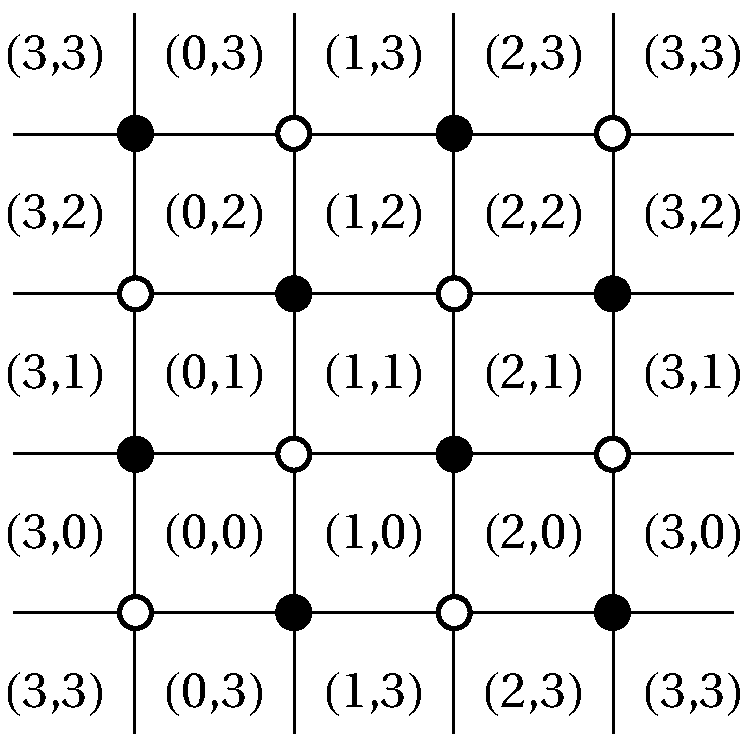
\includegraphics[height=4cm]{coords.pdf}
\caption{Coordinates of the faces }\label{fig:coordsfaces}
\end{figure}

The discrete time index of the Markov chain will be denoted $k=0,1,\,\dots$. We will say that a face $(i,j)$ is \emph{even} if its bottom-left vertex is white, and \emph{odd} otherwise. In the dynamics defined below, the colors of the vertices will interchange at each time step $k$ and we assume that initially the vertex $(0,0)$ is white. Therefore, a face with coordinates $(i,j)$ will be even at time $k$ if $i+j=k\mod 2$ and odd otherwise.


Given a weighting $\ttw$ of the edges, i.e. an assignment of a strictly positive weight to each edge, we first define a deterministic sequence $\{\ttw_k\}_{k\,\ge\,0}$ of edge weightings with $\ttw_0:=\ttw$. To this purpose, note first that the weighting is uniquely defined if we specify the weights of edges on the boundary of every even face. We write then
\[
\ttw_k=\left\{\left(w_{i,j;k}^a, w_{i,j;k}^b, w_{i,j;k}^c,w_{i,j;k}^d\right):
(i,j) \in\bbZ^2, (i+j)=k\hspace{-2mm}\mod
2\right\}
\]
where the 4-tuple of positive numbers
$(w_{i,j;k}^a, w_{i,j;k}^b, w_{i,j;k}^c, w_{i,j;k}^d)$ denotes the edge weights around the face $(i,j)$ at time $k$, where $a,b,c$ and $d$ are the edges labelled clockwise around the face, with $a$ being the topmost horizontal edge on that face. Also for $(i,j) \in \bbZ^2$ and $k \geq 0$, set
\[
\Delta_{i,j;k}= w_{i,j;k}^a w_{i,j;k}^c +w_{i,j;k}^b w_{i,j;k}^d\,.
\]
The relation between $\ttw_k$ and $\ttw_{k+1}$ is, by definition,
\begin{multline}\label{eq:wktowk+1}
\left(w_{i,j;k+1}^a, w_{i,j;k+1}^b, w_{i,j;k+1}^c,w_{i,j;k+1}^d\right)\\
:= \left(\frac{w_{i,j+1;k}^a}{\Delta_{i,j+1;k}}, \frac{w_{i+1,j;k}^b}{\Delta_{i+1,j;k}}, \frac{w_{i,j-1;k}^c}{\Delta_{i,j-1;k}}, \frac{w_{i-1,j;k}^d}{\Delta_{i-1,j;k}} \right)
\end{multline}
for $k\geq 0$ and $(i+j)=k+1\hspace{-2mm}\mod 2$; see Figure~\ref{fig:pesi}.


\begin{figure}
\begin{center}
%[height=6.5cm]
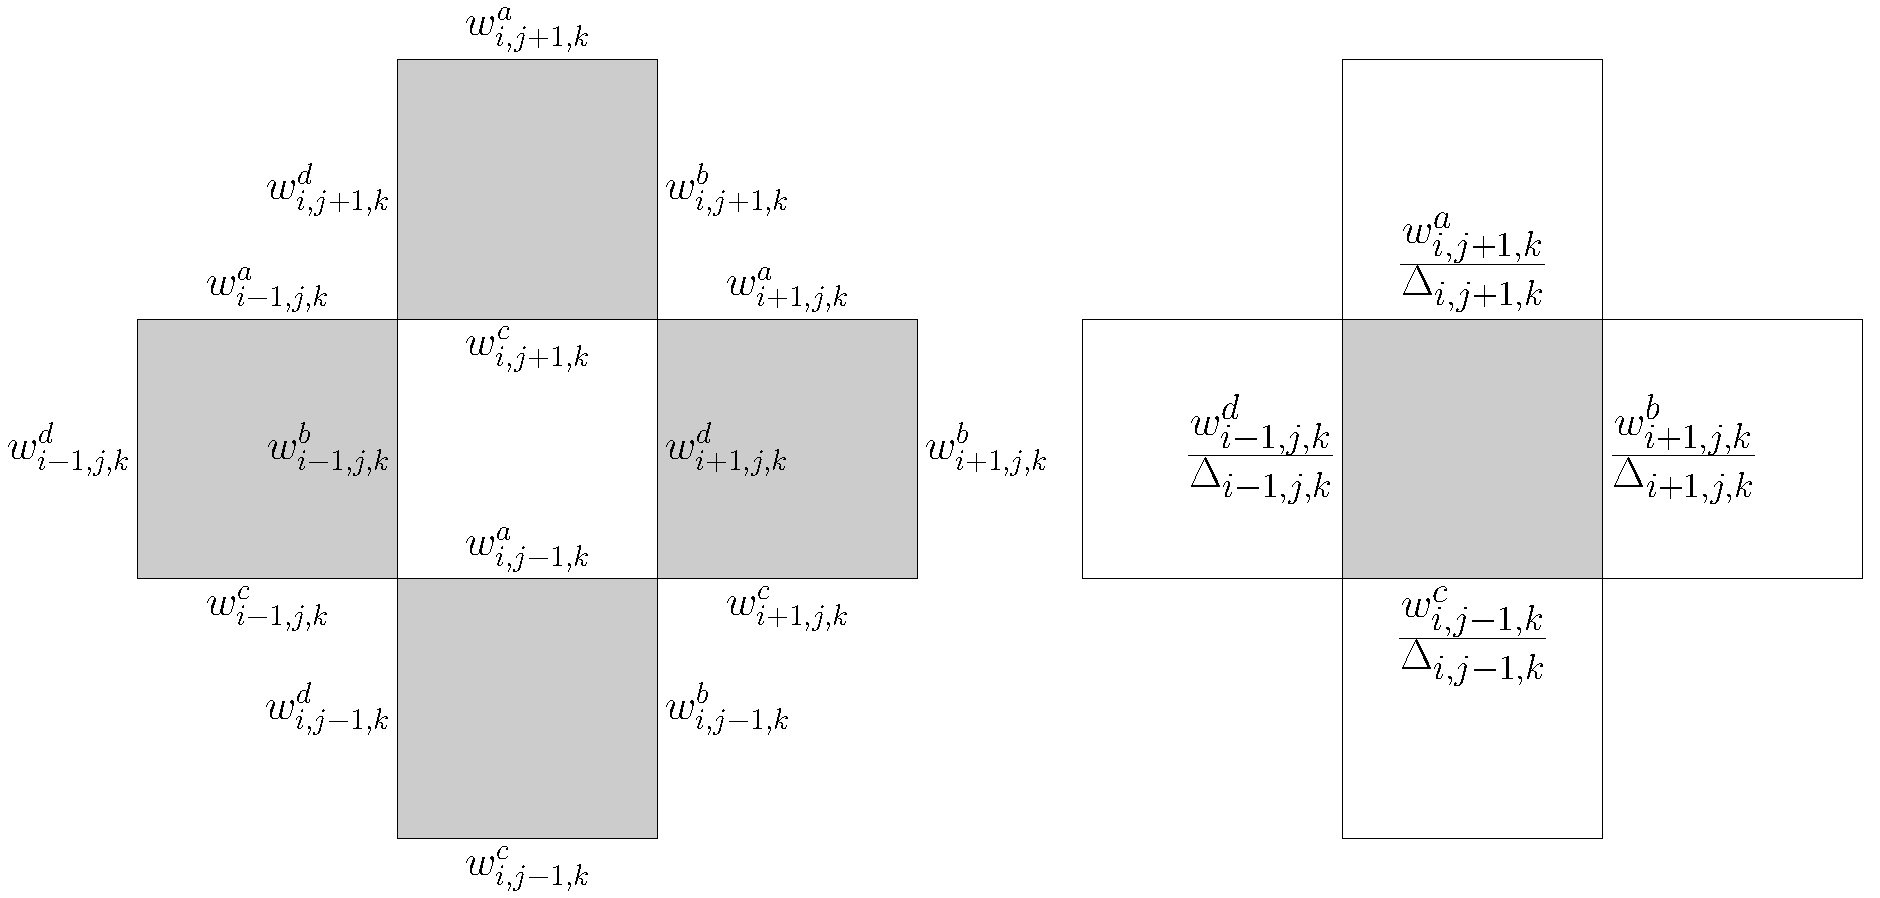
\includegraphics[scale=0.46]{weights1.pdf}
\caption{The left figure shows the weights at time $k$ while the right figure shows the weights at time $k+1$ after applying the shuffling algorithm. In each figure, the shaded squares denote the even faces, at times $k$ and $k+1$ respectively. The central face has coordinates $(i,j)$ with $(i+j)=k+1\mod 2$. }\label{fig:pesi}
\end{center}
\end{figure}



We are now ready to define the shuffling algorithm. This is a discrete-time Markov chain on $\Omega$, the set of dimer coverings, or perfect matchings, of $\bbZ^2$. That is, each $\eta\in\Omega$ is a subset of edges of $\bbZ^2$, such that each vertex is contained in exactly one of them. Each edge contained in $\eta$ will be said to be ``occupied by a dimer''. The chain is not time-homogeneous, since the transition rates depend on the time index $k$, via the edge weights $\ttw_k$. For $k\geq 0$, we define a random map $\Omega\ni \eta \mapsto {T_{k+1}}(\eta)\in\Omega$ through the following four steps, cf. Figure~\ref{fig:spiderconfigs} (only the third one is actually random):
\begin{figure}
\begin{center}
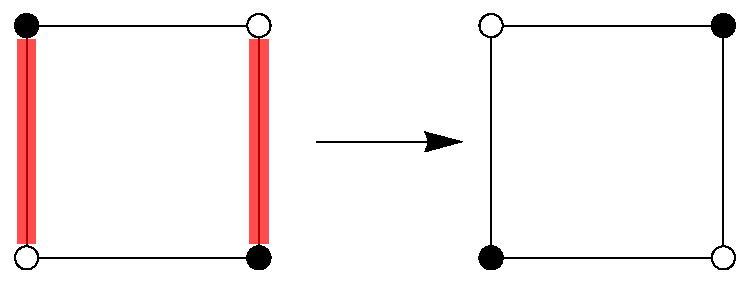
\includegraphics[height=2cm]{shuffle2.pdf}
\hspace{15mm}
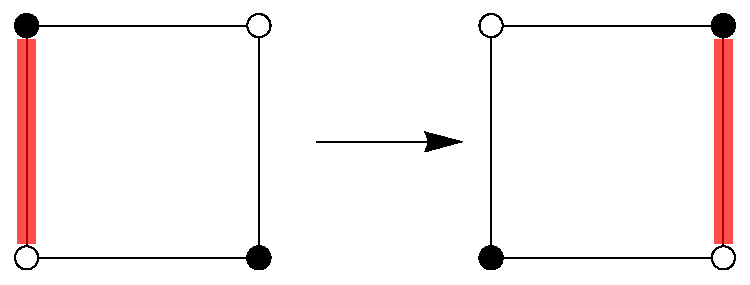
\includegraphics[height=2cm]{shuffle1.pdf}
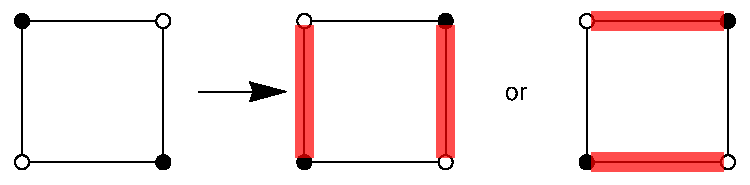
\includegraphics[height=2cm]{shuffle3.pdf}
\caption{The four steps of the dynamics applied to an even face for the three different possibilities (up to rotations) of boundary edges at that face.}\label{fig:spiderconfigs}
\end{center}
\end{figure}


\begin{itemize}
\item [(Deletion step)] All pairs of parallel dimers of $\eta$ covering two of the four boundary edges of any face that is even (at time $k$) are removed.
\item [(Sliding step)] For every even face (at time $k$) with only one boundary edge covered by a dimer of $\eta$, slide this dimer across that face.
\item [(Creation step)] For each face that is even at time $k$ (call $(i,j)$ its coordinates), if there are no dimers of $\eta$ covering any of its four boundary edges, add two parallel vertical dimers to the face with probability
\begin{align*}
&\frac{w^{b}_{i,j;k} w^{d}_{i,j;k}}{\Delta_{i,j;k}}
\\
\intertext{or two parallel horizontal dimers with probability}
&\frac{w^{a}_{i,j;k} w^{c}_{i,j;k}}{\Delta_{i,j;k}}
\end{align*}
(the operations are performed independently for each $(i,j)$ and $k$).
\item[(Interchange step)] Interchange the white and black colors of vertices of the graph.
\end{itemize}
It is well known, and easy to check, that $T_k(\eta)\in\Omega$ if $\eta\in\Omega$. The swapping of colors at each step, that may seem to be pointless at this stage, will appear more natural in the discussion below of the evolution of the height function.

The maps $T_k$ are independent but not identically distributed, since the edge weights depend on $k$. Iteratively applying these maps and letting
\[
\eta_k:=T_{k}\circ\,\dots\,\circ T_1(\eta_0),
\]
one obtains the desired Markov chain $\{\eta_k\}_{k\,\ge\,0}$ on $\Omega$.

\subsubsection{Height function and its evolution}
Each dimer configuration $\eta\in \Omega$ is in one-to-one correspondence (up to a height offset) with a height function $h_\eta(\cdot)$ which is defined on the faces of $\bbZ^2$~\cite{KenLectures}. That is, one fixes the height to be zero at some reference face $f_0$ and one defines the height gradients as
\begin{equation}\label{eq:hgrad}
h_\eta(f')-h_\eta(f)=\sum_{e\sim C_{f\,\to\,f'}}\sigma_e (\dsun_{e\,\in\,\eta}-1/4)
\end{equation}
where the sum runs over the edges crossed by a nearest-neighbor path $C_{f\to f'}$ from $f$ to $f'$, $\dsun_{e\,\in\,\eta}$ is the indicator that $e$ is occupied by a dimer and $\sigma_e=+1$ or $-1$ according to whether $e$ is crossed with the white vertex on the right or left. The r.h.s. of~\eqref{eq:hgrad} is well-known to be independent of the choice of $C_{f\,\to\,f'}$.


In order for the shuffling algorithm to define a Markovian evolution of the height profile, we have to complement the definition of the maps $T_k$ with a prescription of how the height offset evolves as time $k$ increases. The convention that we adopt here is slightly different from that of~\cite{CT:18,zhang2018domino}. We start with the following observation, which is immediately verified from the definition of $T_k$ and of the height function (recall that vertex colors are swapped at each step). Let $f,f'$ be any two faces that are odd at time $k$, i.e. they have coordinates $(i,j)$ and $(i',j')$ respectively, with $i+j=k+1\mod 2$ and $i'+j'=k+1\mod 2$; then,
\[
h_{T_{k+1} (\eta)}(f)-h_{T_{k+1}(\eta)}(f')=h_{\eta}(f)-h_{\eta}(f').
\]
Therefore, we make the following choice:
\begin{defi}\label{def:ho}
If $f$ is an odd face at time $k$, then
\begin{equation}\label{eq:ch1}
h_{T_{k+1} (\eta)}(f)=h_{\eta}(f).
\end{equation}
\end{defi}

This convention fixes unambiguously the whole height function of $\eta_{k+1}$ and in particular the value of $h_{T_{k+1}(\eta)}(f)$ for \emph{even} faces $f$. Namely, let $f$ be any face and let $\eta|_{\partial f}$ (resp. $T_{k+1}(\eta)|_{\partial f}$) be the restriction of the dimer configuration $\eta$ (resp. $T_{k+1}(\eta)$) to the four boundary edges of $f$. Then, one may check by direct inspection starting from the definition of $T_{k+1}$ that, if $f$ is even at time $k$, then
\begin{equation}\label{eq:ch2}
h_{T_{k+1} (\eta)}(f)-h_{\eta}(f)= \frac{ H[\eta]+H[T_{k+1}(\eta)]-V[\eta]-V[T_{k+1}(\eta)]}4,
\end{equation}
where (denoting $e_1,\,\dots\,e_4$ the four boundary edges of $f$, labeled clockwise from the top one),
\begin{equation}\label{eq:hor}
H[\eta]=\dsun_{e_1}(\eta)+ \dsun_{e_3}(\eta)
\end{equation}
and
\begin{equation}\label{eq:vert}
V[\eta]=\dsun_{e_2}(\eta)+ \dsun_{e_4}(\eta);
\end{equation}
see Figure~\ref{fig:spiderheights}.


\begin{figure}
\begin{center}
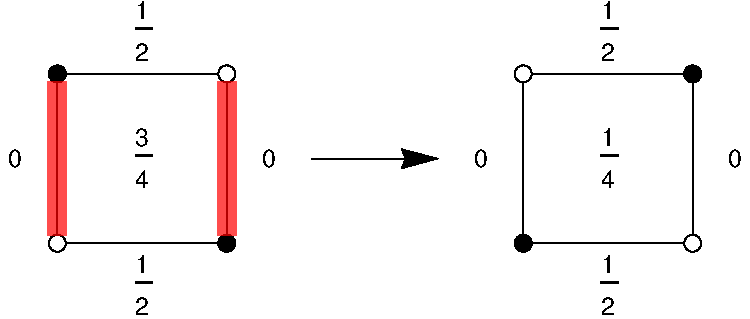
\includegraphics[height=2.5cm]{shuffle1height.pdf}
\hspace{15mm}
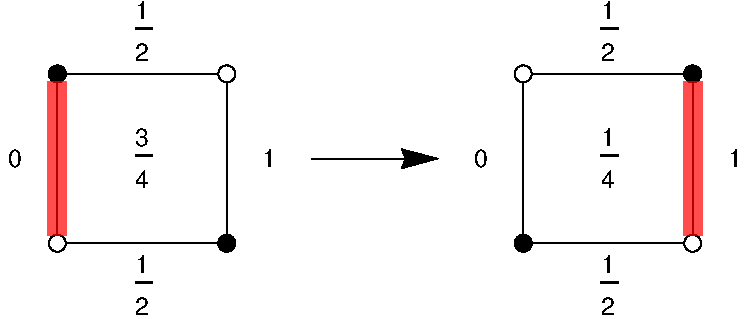
\includegraphics[height=2.5cm]{shuffle2height.pdf}
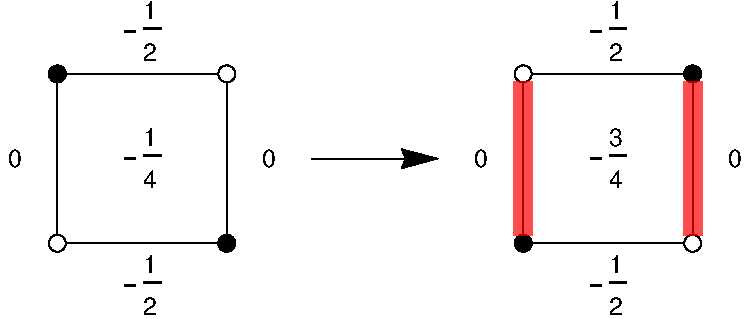
\includegraphics[height=2.5cm]{shuffle3height.pdf}
\caption{The height function change at even faces for configurations only concerning vertical dimers. One can easily obtain the same picture for horizontal edges, by rotating each configuration by $\pi/4$, interchanging the white and black vertices (and as a result multiplying all heights by $-1$). }\label{fig:spiderheights}
\end{center}
\end{figure}



\subsection{Periodic weights}\label{sec:pwat}

In this section, we introduce briefly some of the main aspects of the dimer model machinery needed for the formulation of the main result. Since we are interested in stochastic growth in a translationally invariant situation, here we specialize to the case where the edge weights are periodic in both directions of space. Let the fundamental domain $D_{0,0}$ of size $2n\times 2n, n\in\bbN$, consist of the vertices $\{(i,j): 0 \linebreak\leq i,j \leq 2n-1
\}$, half of which are black and half white. For $ 0 \leq j \leq 2n-1$, the vertices $(2n,j)$ are identified with the vertices $(0,j)$ but are on the fundamental domain $D_{1,0}$ (obtained from $D_{0,0}$ via a horizontal translation by $2n$), while for $0 \leq i \leq 2n-1$, the vertices $(i,2n)$ are identified with the vertices $(i,0)$ but on the fundamental domain $D_{0,1}$. The edge weights are chosen on all edges on $D_{0,0}$ and its boundary edges and then extended by periodicity to the whole graph. Call this weighting $\ttw_0$.


Underlying the dimer model theory is the {characteristic polynomial} $P$. To define $P$, consider $D_{0,0}$ embedded on a $2n\times 2n$ torus as above and let $\wt(x,y)$ denote the weight of the edge $(x,y)$ for two vertices $x$ and $y$ of $D_{0,0}$. Given $z,w\in \bbC$, define $K(z,w)$ to be the Kasteleyn matrix with rows indexed by white vertices and columns indexed by black vertices of $D_{0,0}$, with
\[
(K(z,w))_{xy} =\begin{cases}
\wt(x,y)z^a & \text{if }  (x,y) \text{ is a horizontal edge,}\\
\rmi \,\wt(x,y) w^b & \text{if } (x,y) \text{ is a vertical edge,}\\
0 & \text{if }  (x,y) \text{ is not an edge}
\end{cases}.
\]
where $x$ is a white vertex and $y$ is black vertex in $D_{0,0}$, and
\[
a= 
\begin{cases}
1 & \text{if }x=(2n-1,k)\text{ and }y=(0,k)\\
-1 & \text{if }x=(0,k)\text{ and }y=(2n-1,k)\\
0 & \text{otherwise}
\end{cases}
\]
and
\[
b=
\begin{cases}
1 & \text{if }x=(l,2n-1)\text{ and }y=(l,0)\\
-1 & \text{if }x=(l,0)\text{ and }y=(l,2n-1)\\
0 & \text{otherwise}
\end{cases}
\]
for $0 \leq k,l \leq 2n-1$. The Laurent polynomial $P(z,w)=\det K(z,w)$ is called ``characteristic polynomial''~\cite{KOS03}. Of course, $P$ depends on $n$ and on the weights.

From~\cite{KOS03}, the Newton Polygon (depending on $n$) is defined to be
\[
N(P)=\text{convex hull}\left\{ (j,k) \in \bbZ^2\middle|z^j w^k \text{ is a monomial in }P(z,w) \right\}\subset \bbR^2.
\]
One can check, for the $K(z,w)$ specified above, that $N(P)$ is the (closed) square with vertices $(\pm n,0),(0,\pm n)$.


A probability measure $\mu$ on $\Omega$ is said to be an ergodic Gibbs measure (corresponding to the edge weights $\ttw_0$) if:
\begin{itemize}
\item it is invariant and ergodic with respect to horizontal/vertical translations by multiples of $2n$;
\item it satisfies the following Dobrushin--Lanford--Ruelle (DLR) property. Given any finite subset $\Lambda$ of edges and any dimer configuration $\bar \eta\in \Omega$, let $\Omega_{\Lambda,\bar \eta}$ be the (finite) set of dimer configurations $\eta\in\Omega$ that coincide with $\bar\eta$ outside $\Lambda$. Then, conditionally on $\eta=\bar \eta$ outside $\Lambda$, the $\mu$-probability of a configuration $\eta$ is proportional to the product
\[
\prod_{e\,\in\,\eta\,\cap\,\Lambda} \ttw_0(e)
\]
of $\ttw_0$-weights of the edges in $\Lambda $ occupied by dimers.
\end{itemize}

%%problème du stackrel qui créée une division de ligne dans le paragraphe!
Thanks to translation invariance, one may associate to each ergodic Gibbs measure $\mu$ an average slope $\rho=(\rho_1,\rho_2)$. Here, $\rho_1$ (resp. $\rho_2$) is the expected height difference between a face in $D_{0,0}$ and its translate in $D_{1,0}$ (resp. $D_{0,1}$). The slope $\rho$ is contained in the Newton polygon $N(P)$. Moreover, provided that $\rho$ belongs $\overset{\circ}{N(P)}$, the interior of $N(P)$, there exists a unique Gibbs measure with slope $\rho$~\cite{KOS03} and we denote it by $\pi_{\rho,\ttw_0}$. This measure is known to be determinantal, in the sense that the probability that $r$ given edges $e_1,\,\dots,\,e_r$ belong to $\eta$ is given by the determinant of an $r\times r$ matrix, whose entries are elements of the so-called inverse Kasteleyn matrix.

Define the Ronkin function associated to $P$ as
\begin{align}\label{eq:Ronkin}
R(B)= \frac{1}{(2\pi \rmi)^2} \int \int_{\substack{ |z|=e^{B_1} \\ 
w|=e^{B_2}}} \log |P(z,w)| \frac{dz}{z} \frac{dw}{w}
\end{align}
for $B=(B_1,B_2)\in\bbR^2$. From~\cite{KOS03}, $R$ is the Legendre transform of the so-called surface tension $\sigma$ of the dimer model with the given periodic weights, i.e.
\begin{equation}\label{eq:sigma}
\sigma(\rho)=\sup_{B\,\in\,\bbR^2}(-R(B)+\rho\cdot B).
\end{equation}
We will recall later the relation between $\sigma$ and the ``limit shapes'' of the dimer model.

We write $ \stackrel\circ{N(P)}$, the interior of the Newton polygon, as the disjoint union of $\clR$ (rough region) and $\clS$ (smooth region), whose definition we recall now. (Rough (resp. smooth) phases are called ``liquid'' (resp. ``gaseous'') phases in~\cite{KOS03}.)
From~\cite{KOS03}, it is known that if $\rho\in \stackrel\circ{N(P)}$, two cases can occur:
\begin{itemize}
\item either the measure $\pi_{\rho,\ttw_0}$ is \emph{rough}, meaning that height fluctuations of $h_\eta(f)\linebreak-h_{\eta}(f')$ grow logarithmically w.r.t. the distance between the faces $f,f'$. More precisely,
\begin{equation}
{\Var}_{\pi_{\rho,\ttw_0}}\left(h_\eta(f)-h_{\eta}(f')\right)\sim \frac1{\pi^2}\log \left|f-f'\right|
\end{equation}
as the distance $|f-f'|$ between $f$ and $f'$ diverges. Moreover, the scaling limit of the height profile is a Gaussian Free Field~\cite{KenLectures}. We call $\clR$ the set of such ``rough slopes'';
\item or the measure $\pi_{\rho,\ttw_0}$ is \emph{smooth}, meaning that height fluctuations of $h_\eta(f)\linebreak-h_{\eta}(f')$ have uniformly bounded variance. In this case, $\sigma$ has a cone singularity (i.e. $\nabla\sigma$ is discontinuous) at this value of $\rho$. The set of ``smooth slopes'' is denoted $\clS$.
\end{itemize}
{In both cases, $\sigma(\cdot)$ is strictly convex.}

From~\cite{KOS03}, it is further known that $\clS$ is a finite set and moreover
\begin{equation}\label{eq:rough}
\clS\subset \Bigl[\stackrel\circ{N(P)}\cap \;\bbZ^2\Bigr];
\end{equation}
for generic edge weights $\ttw_0$, $\clS$ actually coincides with the whole $\stackrel\circ{N(P)}\cap \;\bbZ^2$, which contains $2n(n-1)+1$ points. However, this may fail for particular choices of weights: for instance, when all edge-weights are equal, then it is known that $\clS=\emptyset$.



\subsubsection{Shuffling algorithm with periodic weights}

A remarkable feature of the shuffling algorithm is the following (see for instance \cite[Proposition~3.1]{CT:18} and~\cite[Proposition~2.2]{zhang2018domino}):
\begin{prop}\label{prop:misuramappata}
If the initial condition $\eta_0$ at time $0$ is drawn from $\pi_{\rho,\ttw_0}$ (i.e., $\eta_0\sim \pi_{\rho,\ttw_0}$), then at time $k$ one has $\eta_k\sim \pi_{\rho,\ttw_k}$.
\end{prop}

If we had not swapped vertex colors at each step, the slope $\rho$ would swap to $-\rho$ at each step. There are two observations that we will need going forward. The first one is that the characteristic polynomial only changes by a multiplicative constant factor when the weights $\ttw_k$ are replaced by $\ttw_{k+1}$~\cite{GK13} In particular, in view of~\eqref{eq:Ronkin} and~\eqref{eq:sigma}, this implies that the surface tension $\sigma(\cdot)$ for weights $\ttw_k$ equals that for weights $\ttw_{k+1}$, up to an additive constant. Another consequence is the following: since the rough or smooth nature of $\pi_{\rho,\ttw}$ depends on $\ttw$ only through the zeros of the characteristic polynomial $P(z,w)$ on the torus $\{z,w\in \bbC: |z|=|w|=1\}$~\cite{KOS03}, we deduce that $\pi_{\rho,\ttw_{k+1}}$ is rough (resp. smooth) iff $\pi_{\rho,\ttw_{k}}$ is. In other words, the condition $\rho\in \clR$ does not depend on $k$.

Another important observation is the following: even though weights $\ttw_0$ (and therefore $\ttw_k$) are periodic \emph{in space}, the sequence $\{\ttw_k\}_{k\,\ge\,0}$ is in general
\emph{not periodic} w.r.t. the time index $k$. Time-periodicity can, however, hold for special choices of $\ttw_0$ and indeed the cases studied in~\cite{CT:18,zhang2018domino} are time-periodic.



\subsection{The Aztec diamond}
\label{sec:Azteco}
The Aztec diamond $A_N$ of size $N$ is the subset of the graph $\bbZ^2$ whose vertices have Cartesian coordinates $(x_1,x_2)$ satisfying the condition $|x_1-1/2|+|x_2-1/2| \leq N$. We let $E^+_N$ denote the set of edges outgoing from $A_N$, $F^+_N$ the set of faces not in $A_N$ but neighboring $A_N$ and $F_N$ the set of internal faces of $A_N$.


\begin{figure}
\begin{center}
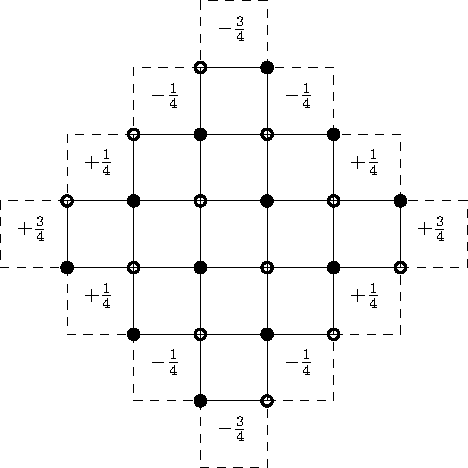
\includegraphics[height=6cm]{Azteco.pdf}
\caption{The Aztec diamond $A_3$ (full edges and colored vertices). The dashed edges are the boundary edges in $E^+_3$ and the faces containing dashed edges are the faces in $F^+_3$. The height function on $F^+_3$ is given.}\label{fig:Azteco}
\end{center}
\end{figure}

Let $\pi_{\ttw,N}$ be the probability measure on $\Omega_N$, the set of perfect matchings of $A_N$, where the weight of a configuration is proportional to the product of the $\ttw$-weights of edges occupied by dimers. Since all vertices of $A_N$ are matched among themselves, all edges in $E^+_N$ are empty and therefore the height difference between two faces in $F^+_N$ is independent of the choice of $\eta\in\Omega_N$. We assume that the coloring of the vertices is such that the vertex of coordinates $(-N+1,1)$ is white. We fix the height offset as in Figure~\ref{fig:Azteco}, by setting the height to $+N/4$ on the leftmost face of $F^+_N$; then, the boundary height ranges from $-N/4$ to $+N/4$.

The height function in $A_N$ satisfies a limit shape phenomenon (or law of large numbers) as $N\to\infty$. Namely, rescale the lattice mesh by $1/(2nN)$ and call $\hat A_N$ the rescaled Aztec diamond (and correspondingly denote $\hat E_N^+,\hat F_N^+,\hat F_N$ the analog of $E_N^+,F_N^+,F_N$). The union of the faces of $\hat A_N$ tends to the square
\begin{equation}\label{eq:Q}
Q=\left\{(x_1,x_2):|x_1|+|x_2|\le 1/(2n)\right\}.
\end{equation}
Define the rescaled height function $\hat h_\eta:\hat F_N\mapsto \bbR$ as
\[
\hat h_\eta(\hat f):=\frac1N h_\eta(f),
\]
with $f\in F_N$ the face of $A_N$ that corresponds to $\hat f$ before rescaling. Thanks to the factor $2n$ in the rescaling, $\hat h_\eta$ is a Lipschitz function whose gradient is contained in the Newton polygon $N(P)$. Note that, if $\hat f=\hat f_N$ is a face in $\hat F^+_N$ whose center tends to $x=(x_1,x_2)\in \partial Q$ as $N\to\infty$, then
\begin{equation}\label{eq:partialQ}
\hat h_\eta(\hat f)\stackrel{N\to\infty}= \psi_{\partial Q}(x):=\frac n2\left({|x_1|-|x_2|}\right).
\end{equation}
The limit shape theorem (cf.~\cite{CKP01} for the model with uniform weights and~\cite{kuchumov2017limit} for the general periodic case) states that there exists a Lipschitz function $\psi_{\ttw}:Q\mapsto \bbR$ that coincides with $\psi_{\partial Q}$ on $\partial Q$, such that for every $\delta>0$,
\begin{equation}\label{eq:lln}
\lim_{N\to\infty} \pi_{\ttw,N}\left(\exists \hat f\in \hat F_N:\left| \hat h_\eta(\hat f)-\psi_{\ttw}(\hat f)\right|>\delta\right)=0.
\end{equation}
Here, with some abuse of notation, $\psi_{\ttw}(\hat f)$ means $\psi_{\ttw}$ computed at the center of the face $\hat f$. The ``limit shape'' $\psi_{\ttw}$ is characterized by being the unique minimizer of the surface tension functional
\[
\int_Q \sigma(\nabla \psi) dx
\]
among Lipschitz functions that equal $\psi_{\partial Q}$ on the boundary. While the boundary condition does not depend on $\ttw$, the limit shape does (through the surface tension), but $\psi_{\ttw_{k+1}}=\psi_{\ttw_{k}}$ because, as we already mentioned, $\sigma$ changes only by an additive constant when $\ttw_k$ is changed into $\ttw_{k+1}$.


\subsection{Statement of Main theorem}
Our main result concerns the average speed of growth for the Markov process in the infinite graph, started from $\pi_{\rho,\ttw}$. By definition, this is given by the limit (provided it exists)
\begin{equation}\label{eq:prov}
v_{\ttw}(\rho):= \lim_{k\to\infty}\frac1k \sum_{j=1}^k\left(\bbE_{\pi_{\rho,\ttw}}\left(h_{\eta_j}(f)\right)-\bbE_{\pi_{\rho,\ttw}}\left(h_{\eta_{j-1}}(f)\right)\right)
\end{equation}
with $f$ any face of $\bbZ^2$ and $\bbE_\nu$ the law of the process started from the probability measure $\nu$. Note that every second term in the sum is zero because every second time the face $f$ is odd.

Since $\eta_j\sim \pi_{\rho,\ttw_j}$ with $\ttw_0\equiv \ttw$, each non-zero term in the sum could in principle be computed via~\eqref{eq:ch2} and Kasteleyn theory, using the determinantal structure of the measure $\pi_{\rho,\ttw_k}$. Following this route, however, it is not clear how to get any manageable expression or to prove that the limit $k\to\infty$ in~\eqref{eq:prov} even exists. One reason is that, for generic periodic weights, it is hard to invert the infinite-volume Kasteleyn matrix explicitly. Fortunately, an alternative way exists, that leads to:

\begin{theo}\label{th:1}
For every $\rho\in\stackrel\circ{N(P)}$ and positive periodic weighting $\ttw$, there exists $v=v_{\ttw}(\rho)$ such that, for any face $f\in \bbZ^2$,
\begin{equation}\label{eq:v}
\lim_{k\to\infty}\frac1k\bbE_{\pi_{\rho,{\ttw}}} \left(h_{\eta_{k}}(f)-h_{\eta_{0}}(f)\right)=v_{\ttw}(\rho).
\end{equation}


The speed $v_{\ttw}(\cdot)$ is determined as follows: let $\psi_{\ttw}(\cdot)$ be the limit shape for the dimer model in the Aztec diamond with weights $\ttw$ and let $x_{\ttw}(\rho)\in \stackrel\circ Q$ (the interior of the unit square in~\eqref{eq:Q}) be a point such that $\nabla \psi_{\ttw}(x_{\ttw}(\rho))=\rho$. Then
\begin{equation}\label{eq:chiev}
v_{\ttw}(\rho)=\psi_{\ttw}(x_{\ttw}(\rho))-x_{\ttw}(\rho)\cdot \rho.
\end{equation}

On the rough region $\clR$, $v_{\ttw}(\cdot)$ is $C^\infty$and $\det(D^2 v_{\ttw})< 0$. On the other hand, $D v_{\ttw}$ is discontinuous at every $\rho\in \clS$.
\end{theo}


A few comments are in order:
\begin{itemize}
\item the existence of $x_{\ttw}(\rho)$ is part of the statement. Uniqueness in general fails (the limit shape $\psi_{\ttw}$ may have ``facets'', i.e. open regions where it is affine) but for $\rho\in\clR$, the point $x_{\ttw}(\rho)$ is unique (see Section~\ref{sec:proprieta}).
\item Using smoothness of $v_{\ttw}(\cdot)$ on $\clR$ and~\eqref{eq:chiev}, one sees that
\begin{equation}\label{eq:chieDv}
D v_{\ttw}(\rho)=-x_{\ttw}(\rho).
\end{equation}
Note that the r.h.s. of~\eqref{eq:chiev} looks like (minus) the Legendre transform of $\psi_{\ttw}$, except that there is no infimum over $x$ and in fact neither $v_{\ttw}$ nor $\psi_{\ttw}$ have any definite convexity.
\item It was observed in~\cite{KO07} that the Euler--Lagrange equation satisfied by the limit shape $\psi_{\ttw}$ of dimer models can be written (in the ``rough region'' where the limit shape is $C^2$) in terms of a first-order PDE (``complex Burgers equation'') for a complex pair $(z,w)$ related by the relations $P(z,w)=0$ and $\pi\nabla \psi_{\ttw}=(-\argl(w),\argl(z))$. Locally, these relations give a bijection between $z$ and $\rho=\nabla\psi_{\ttw}$. Then, using~\cite[Section~3]{borodin2018two}, the above Theorem~\ref{th:1} can be complemented by the following statement:
\[
\hat v_{\ttw}(z):=v_{\ttw}(\rho(z))\; \text{ is a harmonic function of } \, z.
\]
\item For a special case of two-periodic weights ($n=1$), it was found via explicit computation in~\cite[Theorem~3.11]{CT:18} that the behavior of $v_{\ttw}$ near the unique gas slope $\rho=0$ is of the type
\begin{equation}
v_{\ttw}(\rho)\stackrel{\rho\to0}=|\rho|f_1(\argl(\rho))+|\rho|^3f_3\left(\argl(\rho)\right)+O\left(|\rho|^5\right).
\end{equation}
The absence of the $|\rho|^2$ term can be given an interesting interpretation. In fact, this is a simple consequence of formula~\eqref{eq:chiev} plus the fact that, if $x$ approaches a point $x_0$ on the boundary of the ``facet'' where $\nabla\psi_{\ttw}\equiv 0$, then generically $\psi_{\ttw}(x)-\psi_{\ttw}(x_0)$ vanishes as $|x-x_0|^{3/2}$~\cite{KO07} (this behavior is referred to as ``Pokrovsky--Talapov law''~\cite{pokrovskii1980theory}).
\end{itemize}


\subsubsection{Fluctuations}\label{sec:fluct}
One can further prove that height fluctuations grow slowly (at most logarithmically) in time, as is typical for growth models in the AKPZ universality class. In fact, one has uniformly in $k\ge 1$
\[
\bbP_{\pi_{\rho,\ttw}}\left(\left|h_{\eta_k}(f)-h_{\eta_0}(f) -\bbE_{\pi_{\rho,\ttw}} \left(h_{\eta_k}(f)-h_{\eta_0}(f)\right)\right|\ge u g(k)\right)\le \frac{c}{u^2}
\]
for some constant $c$, where $g(k)=\sqrt{\log(k+1)}$ if $\rho\in\clR$ and $g(k)\equiv 1$ if $\rho\in\clS$. The proof of this fact works the same as in~\cite{CT:18} so we will not add details (the speed of convergence $O(u^{-2})$ was not explicitly stated in~\cite{CT:18}, but it can be immediately extracted from the proof). Note in particular that
\begin{equation}\label{eq:nip}
\bbP_{\pi_{\rho,\ttw}}\left(\left|h_{\eta_k}(f)-h_{\eta_0}(f) -\bbE_{\pi_{\rho,\ttw}} \left(h_{\eta_k}(f)-h_{\eta_0}(f)\right)\right|\ge \delta k\right)\le \frac{c [\log (k+1)]^2}{\delta^2k^2}
\end{equation}
and since the r.h.s. is summable in $k$, one can upgrade~\eqref{eq:v} to the almost-sure convergence, with respect to the joint law of the initial condition and of the process,
\begin{equation}\label{eq:asc}
\lim_{k\to\infty}\frac{h_{\eta_{k}}(f)-h_{\eta_{0}}(f)}k=v_{\ttw}(\rho).
\end{equation}


\section{Identification of the speed of growth} \label{sec:Identification}
\label{sec:proofs}


In this section, we prove existence of the speed and formula~\eqref{eq:chiev}.

\pagebreak
\subsection{General properties of the dynamics}\label{sec:Aztecodyn}

We need two general facts: the dynamics is monotone (it preserves stochastic ordering among height profiles) and it is local (information travels at most ballistically through the system).

Let us start with monotonicity. Given two dimer configurations $\eta,\eta'$, we say that $h_\eta\preceq h_{\eta'}$ if $h_\eta(f)\leq h_{\eta'}(f)$ for every face $f$. Given two initial configurations $\eta_0,\eta'_0$, we can couple the two Markov chains $\{\eta_k\}_{k\,\ge\,0}, \{\eta'_k\}_{k\,\ge\,0}$ in the following way (\emph{global monotone coupling}): for any face $f$, if in both configurations $\eta_{k-1}|_{\partial f}=\eta'_{k-1}|_{\partial f}=\emptyset$, then in the ``creation step'' of the shuffling map $T_k$ we choose the same randomness to decide whether we add two vertical or two horizontal dimers around $f$. Then, the following statement holds (it implies the preservation of stochastic order mentioned above): if $h_{\eta_0}\preceq h_{\eta'_0}$, then the same holds at all later times $k$~\cite[Lemma~2.4]{zhang2018domino}.

As far as locality is concerned the point is that, by the definition of the shuffling algorithm, the value of $h_{\eta_k}(f)$ is completely determined by the height at time $k-1$ at the face $f$ and at its four neighbors (this determines the dimer configuration $\eta_{k-1}$ on $\partial f$), plus the randomness used to create parallel dimers at $f$, if the face is even and $\eta_{k-1}|_{\partial f}=\emptyset $. From this, it is immediate to deduce the following:
\begin{prop}\label{prop:loc}
Let $\eta_0,\eta'_0$ be two dimer configurations whose height coincides on all faces at $\ell_1$-distance up to $N+1$ from a given face $f$. Couple the Markov chains started from $\eta_0,\eta'_0$ via the global monotone coupling. Then, $h_{\eta_k}(f)=h_{\eta'_k}(f)$ for every $k\le N$.
\end{prop}

Let us also describe in some more detail how the shuffling algorithm works on the Aztec diamond (this is the framework where the algorithm was originally introduced~\cite{EKLP92,EKLP92b,Pro03}). In a step of the algorithm, a dimer configuration $\eta$ on $A_N$ is mapped to a configuration $\eta'$ on the larger domain $A_{N+1}$. Suppose that we have $\eta_{N}\in\Omega_{N}$, i.e. a dimer configuration on the diamond of size $N$. We can also view $\eta_{N}$ as a subset of edges of $A_{N+1}$ (but not a perfect matching, since the boundary vertices are necessarily unmatched). To construct $\eta_{N+1}$, apply the map $T_{N+1}$ in $A_N$ to $\eta_{N}$ (with weights $\ttw_N$ as above). Note that the faces in $A_{N+1}$ that are closest to the boundary, i.e. the faces in $F^+_{N}$, are even. It is well known that the resulting dimer configuration $\eta_{N+1}$ is a perfect matching of $A_{N+1}$. Due to the swapping of colors, at the next step the faces in $F^+_{N+1}$ are again even and the procedure goes on.

The analog of Proposition~\ref{prop:misuramappata} in the Aztec diamond is the well known fact that, if we start at time zero with a configuration $\eta_0$ on $A_N$ such that $\eta_0\sim \pi_{\ttw_0,N}$ for certain periodic weights $\ttw_0$, then at time $k$ one has $\eta_k\sim \pi_{\ttw_{k},N+k}$.



There is an important point to be discussed: when we introduced the shuffling algorithm on the infinite lattice, we fixed the evolution of the height offset via Definition~\ref{def:ho}. On the other hand, on the Aztec diamond the height offset is fixed by the requirement that the left-most face in $F^+_k$ has height $k/4$. These two conventions must be compatible, i.e., if we adopt the convention~\eqref{eq:ch2} for the evolution of the height function, then the height on the left-most face of $F^+_k$ must be $k/4$ deterministically. This is easily seen inductively in $k$, as explained in the caption of Figure~\ref{fig:compatibili}.


\begin{figure}
\begin{center}
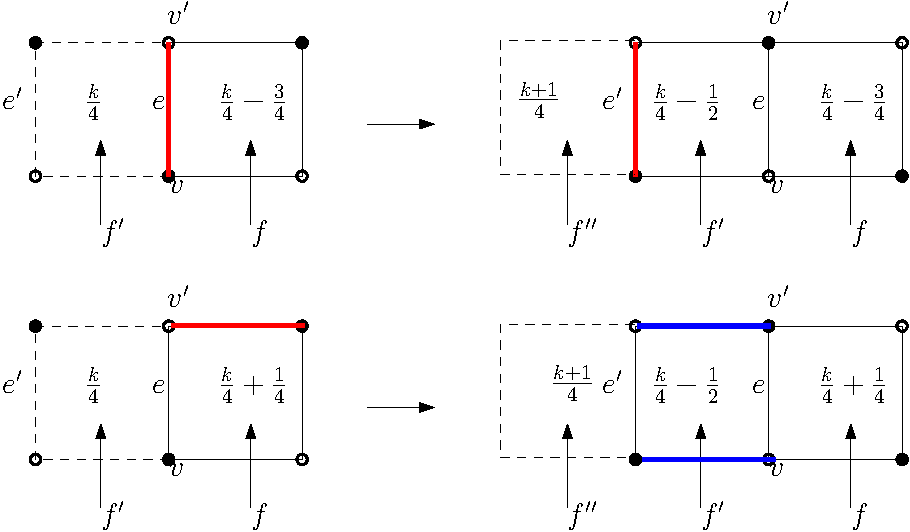
\includegraphics[scale=0.85]{compatibile.pdf}
\caption{Let $f$ be the left-most face of $A_k$ and $f'$ the left-most face of $F^+_k$, where (by inductive assumption) the height is equal to $k/4$. Suppose (top drawing) that $v,v'$ are matched in $\eta_k$. Then, in the application of $T_{k+1}$ the red dimer slides to edge $e'$ and vertex colors are swapped. Since $f$ is odd at time $k$, its height is unchanged and as a consequence the height at $f''$ (the left-most face in $F^+_{k+1}$) is $(k+1)/4$ as it should be. If instead $v'$ is not matched with $v$ (bottom drawing) then $\eta_k$ has no dimer on the boundary of the even face $f'$. Then, in the application of $T_{k+1}$, two parallel dimers (horizontal and drawn in blue in the example of the picture) are created at $f'$. Again, using that the height at the odd face $f$ does not change, one sees that the height at $f''$ is $(k+1)/4$.}\label{fig:compatibili}
\end{center}
\end{figure}



\subsection{The speed of growth}\label{sec:speedo}

Here we prove the following:
\begin{prop}
Let $\rho\in \stackrel\circ{N(P)}$ and assume that there exists $x_{\ttw}(\rho)$ in the interior of $Q$, such that $\psi_{\ttw}(\cdot)$ is $C^1$ in a neighborhood of $x_{\ttw}(\rho)$ and $\nabla\psi_{\ttw}(x_{\ttw}(\rho))=\rho$. Then, the limit in~\eqref{eq:v} exists and~\eqref{eq:chiev} holds.
\end{prop}

The existence of $x_{\ttw}(\rho)$ for every $\rho$ in the interior of the Newton polygon will be proved in the next section.


\begin{proof}
For an integer $N$, let $\bar f_N$ be a face of $A_N$ whose center is at minimal distance from $(2nN) x_{\ttw}(\rho)$. One should think of $N$ as being a large multiple of $k$, the time in~\eqref{eq:v}, with $\epsilon:=k/N$ that will be sent to zero at the end. For later convenience, we let $\Lambda_{N,\epsilon}$ be the square box of side $2k+1$ centered at the face $\bar f_N$. Recall that $A_N$ denotes the $N\times N$ Aztec diamond and take the edge weights to be given by $\ttw$. We run the shuffling dynamics in the Aztec diamond, starting at time zero with the domain $A_N$ and with an initial condition $\tilde \eta_0$ sampled from $\pi_{\ttw,N}$. We denote $\tilde \eta_k$ the configuration at time $k$, where the tilde is used just to distinguish this from the evolution in the infinite graph. The height function of $\tilde\eta_0$ is concentrated at the limit shape $\psi_{\ttw}(\cdot)$. In particular, from~\eqref{eq:lln} with $\delta=\epsilon^2$ we have
\begin{equation}\label{fatica}
\pi_{\ttw,N} \left[\left|h_{\tilde \eta_0}(f)- N \psi_{\ttw}(f/(2nN))\right|\le N \epsilon^2 \text{ for every } f\in \Lambda_{N,\epsilon}\right]\stackrel{N\,\to\,\infty}\to1.
\end{equation}
As before, we identify with some abuse of notation a face $f$ with the point at its center. As observed in Section~\ref{sec:Aztecodyn}, at time $k$, the configuration $\tilde \eta_k$ has law $\pi_{\ttw_k,N+k}$ and we still have~\eqref{fatica} with $N$ replaced by $N+k$. Altogether, we see that
\begin{equation}\label{eq:perA}
\begin{split}
&\bbE_{\pi_{\ttw,N}}\left[\frac{ h_{\tilde \eta_k}(\bar f_N)-h_{\tilde \eta_0}(\bar f_N)}k\right]\\
&=\frac Nk\left[(1+\epsilon)\psi_{\ttw}\left(\frac{x_{\ttw}(\rho)}{1+\epsilon}\right) - \psi_{\ttw}\left(x_{\ttw}(\rho)\right)\right]+O\left(\epsilon^2 \frac Nk\right)\\
&= \psi_{\ttw}(x_{\ttw}(\rho))-x_{\ttw}(\rho)\cdot \rho+o_\epsilon(1)
\end{split}
\end{equation}
where we used that $\nabla\psi_{\ttw}(x_{\ttw}(\rho))=\rho$ and the error term $o_\epsilon(1)$ vanishes as $\epsilon\to0$, since the limit shape is $C^1$ around $x_{\mathtt w}(\rho)$. We also used the fact that $|h_{\tilde \eta_0}|/N, |h_{\tilde \eta_k}|/N$ are uniformly bounded for $k\le \epsilon N$, to deduce from~\eqref{fatica} a statement about their average.

Our goal now is to prove a statement analogous to~\eqref{eq:perA} for the dynamics $\{\eta_k\}_{k\ge0}$ on the infinite graph. By Proposition~\ref{prop:loc}, the evolution of $h_{\eta_j}(\bar f_N),j\le k$ is not influenced by the height function of $\eta_0$ outside $\Lambda_{N,\epsilon}$. Recall that $\eta_0$ is sampled from the infinite-volume measure $\pi_{\rho,\ttw}$. Under this probability measure, the height function is essentially linear, with slope $\rho$ and sub-linear fluctuations. More precisely,
\begin{equation}\label{eq:piatto}
\pi_{\rho,\ttw}\left[\left|h_{\eta_0}(f)-h_{\eta_0}(\bar f_N)-\frac1{2n}\rho\cdot(f-\bar f_N)\right|\le N\epsilon^2 \;\forall\;f\in \Lambda_{N,\epsilon}\right]\stackrel{N\to\infty}\to1
\end{equation}
where once more we have identified a face with its center and the factor $1/(2n)$ is there because $\rho$ is the average height change per fundamental domain. To get~\eqref{eq:piatto}, observe first that
\[
\pi_{\rho,\ttw}\left[h_{\eta_0}(f)-h_{\eta_0}(\bar f_N)\right]=\frac1{2n}\rho\cdot(f-\bar f_N)+O(1),
\]
uniformly in $f\in\Lambda_{\epsilon,N}$ (the error term is there because $f$ is not necessarily an exact translation of $\bar f_N$ in a different fundamental domain). Also, recall that the fourth centered moment of $h_{\eta_0}(\bar f_N)-h_{\eta_0}(f)$ under $ \pi_{\rho,\ttw}$ grows at most like $(\log|\bar f_N-f|)^{2}$ for $|\bar f_N-f|$ large (see~\cite[Section~4]{KOS03} for a $O(\log|\bar f_N-f|)$ bound on the variance; higher moments are treated analogously). Then, a union bound over $f\in \Lambda_{N,\epsilon}$ and an application of Chebyshev's inequality leads to~\eqref{eq:piatto}.

Note that we have not yet specified the height offset $h_{\eta_0}(\bar f_N)$ at time zero. We will fix it in such a way that, with high probability (w.h.p.) as $N\to\infty$,
\begin{equation}\label{eq:then}
h_{\eta_0}(f)\le h_{\tilde \eta_0}(f) \quad \text{for every} \quad f\in \Lambda_{N,\epsilon}.
\end{equation}
For this, note that~\eqref{eq:piatto} implies that w.h.p.
\begin{equation}
h_{\eta_0}(f)\le N\epsilon^2+h_{\eta_0}(\bar f_N)+\frac1{2n}\rho\cdot(f-\bar f_N) \quad \text{for every} \quad f\in \Lambda_{N,\epsilon}
\end{equation}
while~\eqref{fatica} and $C^1$ continuity of the limit shape implies that w.h.p.
\begin{equation}
h_{\tilde \eta_0}(f)\ge N\psi_{\ttw}(x_{\ttw}(\rho))+\frac1{2n}\rho\cdot(f-\bar f_N)+R_{N,\epsilon}
\end{equation}
with $R_{N,\epsilon}/N\epsilon= o_\epsilon(1)$. Then, \eqref{eq:then} holds provided we choose
\[
h_{\eta_0}(\bar f_N)=N\psi_{\ttw}(x_{\ttw}(\rho))-N\epsilon^2-\left|R_{N,\epsilon}\right|.
\]
By monotonicity of the dynamics and Proposition~\ref{prop:loc} we see that $h_{\eta_k}(\bar f_N)\le h_{\tilde\eta_k}(\bar f_N)$ and therefore, w.h.p.,
\begin{equation}
\begin{aligned}
\frac{h_{\eta_k}(\bar f_N)-h_{\eta_0}(\bar f_N)}k&\le \frac1k\left(h_{\tilde\eta_k}(\bar f_N)-N\psi_{\ttw}(x_{\ttw}(\rho))+N\epsilon^2+\left|R_{N,\epsilon}\right|\right)
\\
&\le \frac{h_{\tilde\eta_k}(\bar f_N)- h_{\tilde\eta_0}(\bar f_N)}k+o_\epsilon(1)
\end{aligned}
\end{equation}
where we used~\eqref{fatica} in the last step and $k=\epsilon N$. Note that $[h_{\eta_k}(f)-h_{\eta_0}(f)]/k$ is deterministically bounded by $1$, so we can turn the statement w.h.p. into a statement in average and obtain that
\begin{equation}\label{quasi}
\limsup_{k\to\infty}
\bbE_{\pi_{\rho,\ttw}}\frac{h_{\eta_k}(\bar f_N)-h_{\eta_0}(\bar f_N)}k\le\psi_{\ttw}(x_{\ttw}(\rho))-x_{\ttw}(\rho)\cdot \rho+o_\epsilon(1)
\end{equation}
where we used also~\eqref{eq:perA}. Note that the face $\bar f_N$ depends on the time $k=N\epsilon$. However, since the measure $\pi_{\rho,\ttw}$ is invariant by translations of multiples of $2n$ and the height function has bounded Lipschitz constant, we have~\eqref{quasi} also for any fixed face $f$. Finally, we let $\epsilon\to0$.

A lower bound is proven in the very same way and altogether the statements~\eqref{eq:v} and~\eqref{eq:chiev} follow.
\end{proof}

With similar arguments, we also obtain the following result, that will be useful later:
\begin{prop}\label{prop:damettere}
If there exists $x$ in the interior of $Q$ such that $\psi_{\ttw}$ is $C^1$ in a neighborhood of $x$ and $\nabla\psi_{\ttw}(x)=\rho$ with $\rho=(\rho_1,\rho_2)$ at one of the four corners of the Newton polygon (i.e., $\rho=(\pm n,0)$ or $\rho=(0,\pm n)$) then
\begin{equation}\label{eq:ahah}
\psi_{\ttw}(x)=\rho\cdot x+\frac1{4n}\left(\left|\rho_2|-|\rho_1\right|\right).
\end{equation}
\end{prop}

\begin{proof}
Assume to fix ideas that $\rho=(n,0)$. As above, let $\bar f_N$ be the face of $A_N$ closest to $(2n N) x$, let $k=N\epsilon$ and $\Lambda_{N,\epsilon}$ be the square of side $2k+1$ centered around $\bar f_N$. One has, in analogy with~\eqref{eq:perA} and with the same argument,
\begin{equation}\label{eq:expand}
\frac1{\left|\Lambda_{N,\epsilon}\right|}\sum_{f\,\in\,\Lambda_{N,\epsilon}} \bbE_{\pi_{\ttw,N}}\left[\frac{ h_{\tilde \eta_k}(f)-h_{\tilde \eta_0}(f)}k\right]= \psi_{\ttw}(x)-x\cdot \rho+o_\epsilon(1).
\end{equation}

On the other hand, let $F$ be the collection of faces in $\Lambda_{N,\epsilon}$ (there are approximately $4 k^2$ of them). Write $F=F^{(+,j)}\cup F^{(-,j)}$, where $F^{(+,j)}$ contains the faces that are even at time $j$ and $F^{(-,j)}$ all the others. Because of~\eqref{eq:lln} and the fact that $\nabla\psiw\linebreak =(n,0)+o_\epsilon(1)$ in an $\epsilon$-neighborhood of $x$, from the definition of height function we see that, with probability $1-o_\epsilon(1)$, a proportion $1-o_\epsilon(1)$ of the dimers of $\tilde \eta_0$ in $\Lambda_{N,\epsilon}$ occupy a vertical edge with bottom white vertex. The same holds for $\tilde \eta_j,j\le k$, because $\tilde \eta_j$ has the same limit shape as $\tilde \eta_0$. Therefore, a proportion $1-o_\epsilon(1)$ of the faces in $F^{(+,j)}$ have a single vertical dimer of $\tilde \eta_j$ along their boundary. From~\eqref{eq:ch2} we see that each such even face contributes $-1/2$ to the height change from time $j$ to $j+1$. Since $|F^{(+,j)}|/|F|=1/2+o_\epsilon(1)$, the l.h.s. of~\eqref{eq:expand} equals also $-1/4+o_\epsilon(1)$ and~\eqref{eq:ahah} follows.
\end{proof}


\subsection{The limit shape}
Here we give some analytic properties of the limit shape $\psi_{\ttw}(\cdot)$ and prove the existence of $x_{\ttw}(\rho)$:
\begin{theo}\label{prop:KO}
There exists a non-empty, open subset $\clF$ of the rescaled Aztec diamond $Q$ (cf.~\eqref{eq:Q}) where $\psi_{\ttw}(\cdot)$ is $C^1$ and the gradient
\[\nabla \psi_{\ttw}(\cdot)\in \stackrel \circ{ N(P)}.
\]
For every $\rho\in \stackrel\circ{N(P)}$, there exists $x_{\ttw}(\rho)\in \clF$ such that
\[
\nabla \psi_{\ttw}(x_{\ttw}(\rho))=\rho.
\]
\end{theo}



\begin{proof}[Proof of Theorem~\ref{prop:KO}]
For $x=(x_1,x_2)\in Q$, let
\begin{equation}\label{eq:minmax}
\begin{aligned}
\psi^-(x) &=\max\left[\phi_W(x),\phi_E(x)\right] :=\max\left[-n x_1-\frac14, n{x_1}-\frac14\right] =n{|x_1|}-\frac14,\\
\psi^+(x) &=\min\left[\phi_S(x),\phi_N(x)\right]\:\,:=\min\left[n{x_2}+\frac14,-n{x_2}+\frac14\right] =-n{|x_2|}+\frac14
\end{aligned}
\end{equation}
and note that $\psi^-$ (resp. $\psi^+$) is the minimal (resp. maximal) Lipschitz function with gradient in $N(P)$ that equals $\psi_{\partial Q}$ on $\partial Q.$ We let
\begin{equation}\label{eq:mathcalF}
\clF_0:=\left\{x\in Q: \psi_{\ttw}(x)\ne \psi^\pm(x)\right\}\subset \stackrel \circ Q.
\end{equation}
It is easy to see the following (the proof is given below):
\begin{lemm}\label{lemma:pro}
The set $\clF_0$ is non-empty.
\end{lemm}

We need some regularity properties of the limit shape $\psi_{\ttw}$, and for this we appeal to~\cite{Duse,SS10}. Let us compactify the Newton polygon by introducing a continuous map $H:N(P)\mapsto S^2$ (the two-dimensional sphere) in such a way that $\partial N(P)$ is mapped to a point of $S^2$ while $H$ is a homeomorphism between
\[
\stackrel\circ{N(P)}\text{ and }\,H(\stackrel\circ{N(P)})\,.
\]
Then one has:

\begin{prop}[{\cite[Theorems~4.1 and~1.3]{SS10}\label{prop:compactify}}]
The map $x\mapsto H(\nabla\psi_{\ttw}(x))$ is continuous in the interior of $Q$. Moreover, $\psi_{\ttw}$ is $C^1$ in $\clF_0$.
\end{prop}


Define further the open set
\begin{equation}\label{eq:F0}
\clF: =\{x\in \clF_0:\nabla\psi_{\ttw}(x)\in \;\stackrel \circ{N(P)}\},
\end{equation}
that is the one appearing in the statement of Theorem~\ref{prop:KO}. Decompose $\clF$ as the union of the open set
\begin{equation}\label{eq:Fr}
\clF_R:=\left\{x\in \clF: \nabla\psi_{\ttw}(x)\in \clR\right\}
\end{equation}
and the closed set
\begin{equation}\label{eq:Fs}
\clF_S:=\left\{x\in \clF: \nabla\psi_{\ttw}(x)\in \clS\right\}.
\end{equation}
\begin{prop}\label{prop:notempty}
The set $\clF_R$ is non-empty.
\end{prop}

Let us assume for the moment Proposition~\ref{prop:notempty} (the proof is given below) and let us proceed with the proof of Theorem~\ref{prop:KO}. In general, $ \clF_S$ consists of a collection of disjoint, simply connected sets (these were called ``bubbles'' in~\cite{KO07}); on each bubble, the gradient $\nabla\psi_{\ttw}$ is constant and belongs to one of the finitely many slopes in $\clS$. It is also known~\cite{morrey2009multiple} that, on $ \clF_R$, the limit shape $\psi_{\ttw}$ is not just $C^1$ but actually $C^\infty$, since the surface tension $\sigma(\rho)$ is $C^\infty$ for $\rho\in \clR$. Therefore, in particular, the map $D:x\mapsto \nabla \psi_{\ttw}(x)$ is a $C^1$ map from $\clF_R$ to $\clR$. The next step requires the following:

\begin{theo}[{\cite{Duse}\label{prop:clearly}}]
The map $D:x\mapsto \nabla \psi_{\ttw}(x)$ is a proper map\footnote{\label{foot:natural}
Properness does not hold for general domains $Q$ and boundary values $\psi_{\partial Q}$. Theorem~\ref{prop:clearly} holds for the Aztec diamond because in this case $Q$ is a convex polygonal domain with sides perpendicular to the sides of the Newton polygon, and $\psi_{\partial Q}$ in~\eqref{eq:partialQ} is a ``natural boundary value'' for $Q$. The notion of ``natural boundary value'' is defined in~\cite{Duse} and it requires in particular that, if the side $\ell$ of $Q$ is perpendicular to the side $[p_i,p_{i+1}]$ of the Newton polygon with $p_i,p_{i+1}$ two of its adjacent corners, then the derivative of $\psi_{\partial Q}$ along $\ell$ equals $\langle t_\ell,p_i\rangle$ with $t_\ell$ the tangent vector to $\partial Q$ along $\ell$. } from $\clF_R$ to $\clR$ (i.e. the pre-image of every compact subset of $\clR$ is compact).
\end{theo}

Let us prove that the Jacobian $\det(J(x))$ of the map $D $ is everywhere non-positive on $\clF_R$ and not identically zero. The Jacobian matrix equals
\begin{equation}\label{eq:J}
J(x)=
\begin{bmatrix}
\partial^2_{x_1}\psi_{\ttw}(x)&\partial^2_{x_1 x_2}\psi_{\ttw}(x)\\[0.10em]
\partial^2_{x_1 x_2}\psi_{\ttw}(x)&\partial^2_{x_2}\psi_{\ttw}(x)
\end{bmatrix}.
\end{equation}
On the other hand, on $\clF_R$, $\psi_{\ttw}(\cdot)$ satisfies the Euler-Lagrange equation
\begin{equation}\label{eq:EL}
\sigma_{11}\partial^2_{x_1}\psi_{\ttw}(x)+2 \sigma_{12} \partial^2_{x_1x_2}\psi_{\ttw}(x)+
\sigma_{22} \partial^2_{x_2}\psi_{\ttw}(x)=0,
\end{equation}
with $\sigma_{ab}$ the derivative of $\sigma(\rho)$ w.r.t. the arguments $\rho_a,\rho_b$, computed at $\rho:=\nabla\psi_{\ttw}(x)\linebreak\in\clR$. For $\rho\in \clR$, the matrix $\{\sigma_{ab}\}_{a,b\,=\,1,2}$ is strictly positive definite, in particular $|\sigma_{12}|<\sqrt{\sigma_{11}\sigma_{22}}$. From this, we deduce that
\begin{equation}\label{eq:contorto}
\det(J(x))\ge0\Rightarrow J(x)_{i,j}=0 \quad \text{for every} \quad 1\le i,j\le 2.
\end{equation}
In fact, assume first that $\partial^2_{x_1x_2}\psi_{\ttw}(x)=0$. Then, $\partial^2_{x_1}\psi_{\ttw}(x) \partial^2_{x_2}\psi_{\ttw}(x)\ge0$ (because $\det J(x)\ge0$) but on the other hand~\eqref{eq:EL} reduces to
\begin{equation}\label{eq:ELbis}
\sigma_{11}\partial^2_{x_1}\psi_{\ttw}(x)+
\sigma_{22} \partial^2_{x_2}\psi_{\ttw}(x)=0.
\end{equation}
Since both $\sigma_{11},\sigma_{22}$ are strictly positive, the only possibility is that $\partial^2_{x_1}\psi_{\ttw}(x)\linebreak= \partial^2_{x_2}\psi_{\ttw}(x)=0$. On the other hand, assume (by contradiction) that $\partial^2_{x_1x_2}\psi_{\ttw}(x)\ne0$, so that $\partial^2_{x_1}\psi_{\ttw}(x) \partial^2_{x_2}\psi_{\ttw}(x)>0$. Then
\begin{equation}\label{eq:contr}
\begin{aligned}
0 &\ge \sigma_{11}\partial^2_{x_1}\psi_{\ttw}(x)+\sigma_{22}\partial^2_{x_2}\psi_{\ttw}(x)-2 |\sigma_{12}|\sqrt{\partial^2_{x_1}\psi_{\ttw}(x)\partial^2_{x_2}\psi_{\ttw}(x)}\\
&> \sigma_{11}\partial^2_{x_1}\psi_{\ttw}(x)+\sigma_{22}\partial^2_{x_2}\psi_{\ttw}(x)-2 \sqrt{\sigma_{11}\sigma_{22}}\sqrt{\partial^2_{x_1}\psi_{\ttw}(x)\partial^2_{x_2}\psi_{\ttw}(x)}\ge0
\end{aligned}
\end{equation}
which is a contradiction because the second inequality is strict. Altogether, \eqref{eq:contorto} follows. From this, we see that $\det(J(\cdot))$ can vanish identically on $\clF_R$ only if $\psi_{\ttw}(\cdot)$ is affine, which is clearly not possible in view of Proposition~\ref{prop:clearly}.

We have that the map $D$ is proper and its Jacobian is non-negative and not identically vanishing. Then, by~\cite[Theorem~1]{nijenhuis1962theorem}, we deduce that the map $D$ is onto: for every $\rho\in \clR$, there exists $x_{\ttw}(\rho)\in \clF_R$ with $\nabla \psi_{\ttw}(x_{\ttw}(\rho))=\rho$.



It remains to show the existence of $x_{\ttw}(\rho)$ for every $\rho\in \clS$. Let $\{\rho_i\}$ be a sequence of slopes in $\clR$ that converges to $\rho$. Any limit point $\bar x$ of $x_{\ttw}(\rho_i)$ is in $\clF_0$ (because of Proposition~\ref{prop:clearly}). Due to Proposition~\ref{prop:compactify}, the slope of $\psiw$ at $\bar x$ is $\rho$, so we can set $x_{\ttw}(\rho):=\bar x$.
\end{proof}

We conclude this section by proving the two technical results, Lemma~\ref{lemma:pro} and Proposition~\ref{prop:notempty} that were stated above.

\begin{proof}[Proof of Lemma~\ref{lemma:pro}]
Since $\psi^-(x)<\psi^+(x)$ for every $x$ in the interior of $Q$ and $\psi_{\ttw}$ is continuous, we have just to exclude that $\psi_{\ttw}\equiv \psi^-$ or $\psi_{\ttw}\equiv \psi^+$. Assume for instance that $\psi_{\ttw}\equiv \psi^+$; we are going to exhibit a function $\psi$, with the right boundary value, such that
\begin{equation}\label{eq:atr}
\int_Q \sigma(\nabla\psi)dx<\int_Q\sigma(\nabla\psi_{\ttw})d x=\frac{|Q|}2(\sigma(0,n)+\sigma(0,- n)).
\end{equation}
For this purpose, let for $\epsilon>0$ small
\[
\psi(x):=\min\left(\psi^+(x),4 \epsilon n^2 x_1^2+(1/4-\epsilon)\right).
\]
It is immediate to see that $\psi(x)=4\epsilon n^2 x_1^2+(1/4-\epsilon)$ in
\[
S_\epsilon:=\left\{x:|x_2|\le \frac{\epsilon}{n} \left(1-4n^2 x_1^2\right)\right\}
\]
and $\psi(x)=\psi^+(x)$ in $Q\setminus S_\epsilon$, so in particular $\psi$ equals $\psi_{\partial Q}$ on $\partial Q$. The difference between the r.h.s. and the l.h.s. of~\eqref{eq:atr} is then
\begin{equation}\label{eq:diff}
\int_{S_\epsilon}\left[\frac12\left(\sigma(0,n)+\sigma(0,-n)\right)-\sigma\left(8 \epsilon n^2 x_1,0\right)\right]dx.
\end{equation}
Since $\sigma(\cdot)$ is strictly convex, one has
\[
\frac12\left[\sigma(0,n)+\sigma(0,-n)\right]>\sigma(0,0).
\]
Therefore, using continuity of $\sigma(\cdot)$, for $\epsilon$ small enough the difference~\eqref{eq:diff} is strictly positive and, as a consequence, the minimizer $\psi_{\ttw}$ of the surface tension functional cannot coincide with $\psi^+$.
\end{proof}

\begin{proof}[Proof of Proposition~\ref{prop:notempty}]
We begin by making an observation on the shape of $\clF_0$. Recall from~\eqref{eq:minmax} the definition of $\phi_{a},a\in \{N,E, S, W\}$ and define the (possibly empty) regions
\begin{equation}\label{eq:regcard}
Q_{a}:=\left\{x\in \stackrel \circ Q: \psi_{\ttw}(x)=\phi_a(x)\right\}, \quad a\in \{N,E,S,W\}.
\end{equation}
$Q_N$ belongs to the triangle $\{x\in Q: x_2\ge0\}$, otherwise $\psi_{\ttw}$ would exceed the maximal function $\psi^+$; similar statements hold for $Q_S,Q_E,Q_W$. See Figure~\ref{fig:F}. Also, it follows from~\cite[Theorem~4.2]{SS10} that
\[
\partial Q_N\cap \stackrel\circ Q
\]
is the graph of a concave function; analogously, $\partial Q_a\cap \stackrel\circ Q$ for $a\in\{E,S,W\}$ is the graph of a concave function in a reference frame rotated clockwise by $\pi/4,\pi/2$ and $3\pi/4$ respectively.


\begin{figure}
\begin{center}
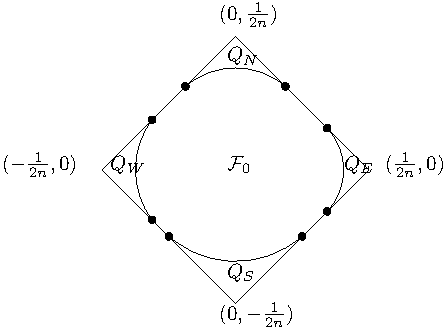
\includegraphics[height=6cm]{F.pdf}
\caption{The square $Q$ with the convex region $\clF_0$ and the four frozen regions $Q_a,a=N,W,S,E$. }\label{fig:F}
\end{center}
\end{figure} Because of the definition of $\psi^\pm$, we see that
\[
\clF_0=\stackrel\circ Q\setminus \cup_{a\,\in\,\left\{N,E,S,W\right\}}Q_a.
\]
Note that $\clF_0$ is convex.



Before proving that $\clF_R$ is non-empty, let us show that $\clF$ is non-empty. Let $\rho^{(a)},\linebreak a\in\{N,E,S,W\}$ be the gradient of $\phi_a(\cdot)$ (these are also the four corners of $N(P)$) and $\ell^{(i)},i\in\{NE,SE,SW,NW\}$ the open segment connecting $\rho^{(N)}$ to $\rho^{(E)}$ etc. Remark that if $x\in \clF_0$, then $\nabla\psi_{\ttw}(x)$ cannot coincide with any of the slopes $\rho^{(a)},\linebreak a\in\{N,E,S,W\}$. In fact, thanks to Proposition~\ref{prop:damettere}, in this case one would have
\[
\psi_{\ttw}(x)=\rho^{(a)}\cdot x+\frac1{4n}\left(\left|\rho^{(a)}_2\right|-\left|\rho^{(a)}_1\right|\right)=\phi_a(x),
\]
which contradicts the fact that $x\in\clF_0$. Therefore, we have that
\begin{equation}\label{eq:FF0}
\clF=\clF_0\setminus \cup_{i\,\in\,\left\{NE,SE,SW,NW\right\}} \clF^{(i)},
\end{equation}
with
\[
\clF^{(i)}=\left\{x\in \clF_0:\nabla\psi_{\ttw}(x)\in \ell^{(i)}\right\}.
\]
In general, the region $\clF$ is a proper subset of $\clF_0$, see Figure~\ref{fig:semifrozen}.


\begin{figure}
\begin{center}
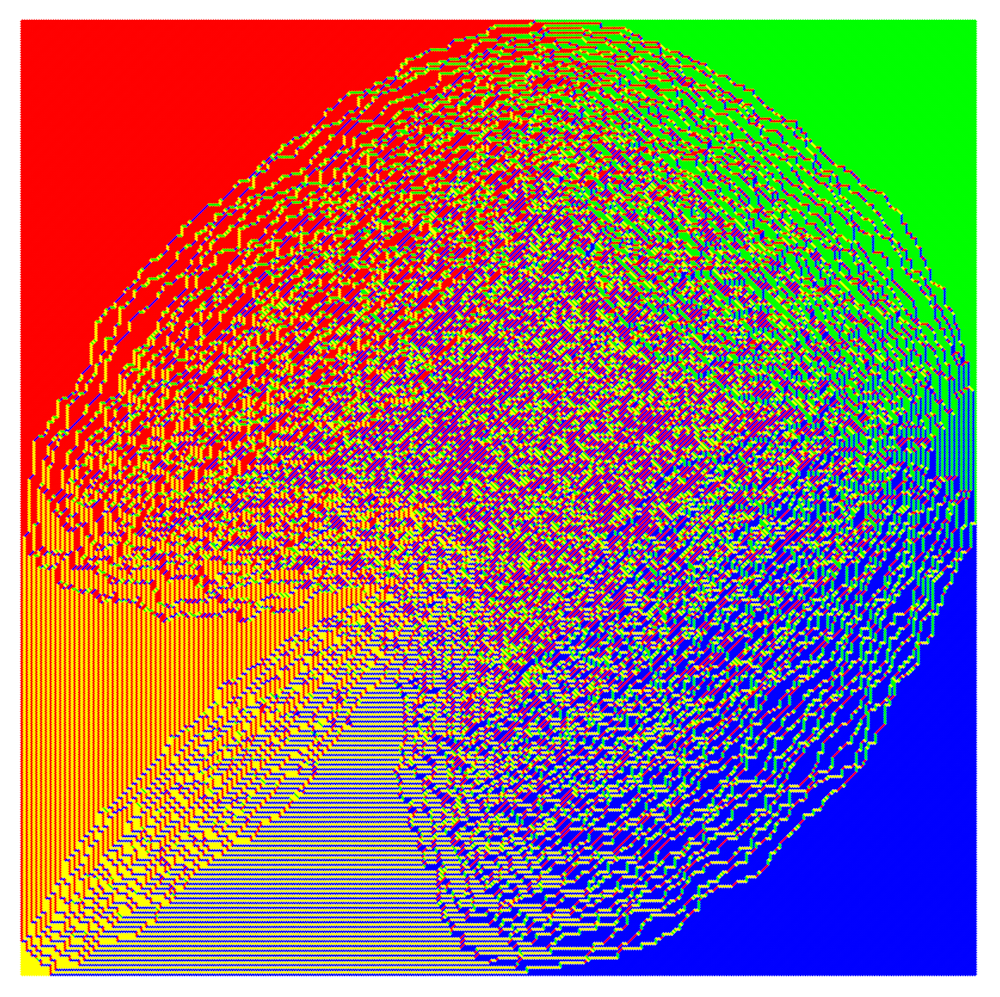
\includegraphics[scale=0.80]{semifrozen.png}
\caption{A random domino tiling of the Aztec diamond of size $N=800$ (rotated by $45$ degrees) with edge weights of period $n=2$ (the weights were randomly chosen on the fundamental domain and then extended by periodicity). The configuration is obtained via the shuffling algorithm and it is therefore a perfect sample from $\pi_{\ttw,N}$. In addition to the frozen regions $Q_N,Q_E,Q_S,Q_W$ adjacent to the corners of the domain, where the gradient of the limit shape $\psi_{\ttw}$ equals $(\pm n,0),(0,\pm n)$, one remarks the presence of regions, adjacent to the sides, where $\nabla\psi_{\ttw}$ belongs to $\partial N(P)\setminus\{(\pm n,0),(0,\pm n)\}$. These regions belong to $\clF_0$ but not to $\clF$. }\label{fig:semifrozen}
\end{center}
\end{figure}


Using also the second statement in Proposition~\ref{prop:compactify}, we conclude that if (by contradiction) $\clF$ is empty, then necessarily $\clF_0$ must coincide with one of the four sets $\clF^{(i)}$. To fix ideas, say that $\clF_0=\clF^{(NW)}$, i.e. everywhere in $\clF_0$, $\nabla\psi_{\ttw}$ is a non-trivial convex combination of $\rho^{(W)}=(-n,0)$ and $\rho^{(N)}=(0,-n)$. Let $\gamma$ be the curve along $\partial \clF_0$ from point $A$ to point $B$, as in Figure~\ref{fig:F2}, and let $t_p$ be the tangent vector at a point $p\in\gamma$.


\begin{figure}
\begin{center}
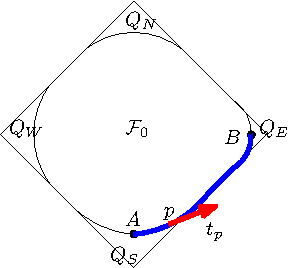
\includegraphics[height=6cm]{F2.pdf}
\caption{The curve $\gamma$ (in blue) and the tangent vector ${t}_p$ at a point $p\in\gamma$.}\label{fig:F2}
\end{center}
\end{figure} From the definition of $Q_S,Q_W$ one has that the directional derivative of $\psiw$ in direction $t_p$ equals $t_p\cdot g_p$, with $g_p\in \ell^{(SE)}$. On the other hand, if $\gamma'$ is a curve from $A$ to $B$ that runs slightly inside $\clF_0$ at distance $\delta$ from $\gamma$, we have that the directional derivative along $\gamma'$ at a point $p'$ equals $t'_{p'}\cdot \nabla\psiw(p')$, with $\nabla \psiw(p')\in \ell^{(NW)}$, because $\clF_0=\clF^{(NW)}$ by assumption. Taking $\delta\to0$, one easily sees that these two facts are not compatible with $\psiw$ being continuous along $\gamma$. This proves that $\clF$ is not empty.

Finally, the fact that $\clF_R\ne\emptyset$ follows easily from $\clF\ne\emptyset$. In fact, if $\clF_R$ were empty, then $\nabla \psi_{\ttw}(x)$ would belong to $\clS$ for every $x\in \clF$ and (because of Proposition~\ref{prop:compactify}) it would actually take a constant value $\bar\rho$ on $\clF$. If $\clF=Q$, this is a contradiction since the affine function with slope $\bar \rho$ cannot match the boundary datum $\psi_{\partial Q}$. If on the other hand $Q\setminus \clF\ne\emptyset$, then take a sequence of points $x_i\in \clF$ and a sequence $y_i \in Q\setminus \clF$ that have the same limit in the interior of $Q$. One has $\nabla\psiw(x_i)=\bar \rho$ while $\nabla\psi(y_i)\in \partial N(P)$, which contradicts Proposition~\ref{prop:compactify}.
\end{proof}


\section{Properties of \texorpdfstring{$v_{\ttw}(\rho)$}{v mathtt w(rho)}} \label{sec:Properties}
\label{sec:proprieta}
We start with the following statement, whose proof is given below:
\begin{prop}\label{prop:vsmooth}
The function $\rho\mapsto v_{\ttw}(\rho)$ is $C^\infty$ on $\clR$.
\end{prop}

\begin{rema}
We know that the determinant of the Hessian matrix $J(x)$ of $\psi_{\ttw}$ is negative or zero on the rough region $\clF_R$; if we knew that the inequality is everywhere strict, $C^\infty$ continuity of $v_{\ttw}(\cdot)$ would easily follow from formula~\eqref{eq:implicit} below and from further derivation w.r.t. $\rho$. On the other hand, non-vanishing of $J(x)$ in the rough region is not a general property of macroscopic shapes of dimer models. For instance, for the dimer model on the honeycomb graph with uniform weights, one can verify from the explicit solution~\cite{CLP98} that the macroscopic shape $\psi$ in a hexagonal domain has a Hessian with strictly negative determinant in the whole rough region, except at a single point (the center of the domain), where all entries of the Hessian matrix are zero. To overcome this problem, for the proof of Proposition~\ref{prop:vsmooth} we will not rely directly on analytic properties of the limit shapes, bur rather on the definition~\eqref{eq:prov} of the speed and on the properties of the dimer measure $\pi_{\rho,\ttw_j}$ under the dynamics $\{\ttw_j\}_{j\ge 0}$ of the edge weights (``spider move dynamics'').
\end{rema}

From Proposition~\ref{prop:vsmooth} and the formula~\eqref{eq:chiev} for the speed, we deduce
\begin{equation}\label{eq:Dv}
D v_{\ttw}(\rho)=-x_{\ttw}(\rho), \quad \rho\in\clR.
\end{equation}
By the way, this shows that $x_{\ttw}(\rho)$ is unique for $\rho$ in the rough region. This formula also allows to prove that the speed is not $C^1$ at smooth slopes. Indeed, we know from Theorem~\ref{prop:KO} that for every $\bar\rho\in \clS$, there exists $x_{\ttw}(\bar\rho)$ in the interior of $Q$, where the slope of $\psiw$ is $\bar\rho$. Moreover, it is known~\cite{Duse} that, since the boundary condition $\psi|_{\partial Q}$ is ``natural'' (cf. Footnote~\ref{foot:natural}), the set $B_{\bar \rho}:=\{x\in Q: \nabla\psiw(x)=\bar \rho\}$ is a closed set with non-empty interior. Letting $x\in \clF_R$ approach different points of $B_{\bar\rho}$ (so that $\nabla\psiw(x)$ approaches $\bar\rho$, by continuity of $x\mapsto \nabla\psiw(x)$), we see from~\eqref{eq:Dv} that $D v_{\ttw}(\rho)$ does not have a unique limit as $\rho\to\bar \rho$.

From~\eqref{eq:Dv} we see also that, for $\rho\in \clR$,
\begin{equation}\label{eq:implicit}
D^2 v_{\ttw}(\rho) = - J(x_{\ttw}(\rho))^{-1},
\end{equation}
where the $2\times 2$ Jacobian matrix $J(\cdot)$ is as in~\eqref{eq:J}. We already know that $\det(J(x))\linebreak\le0$, and the fact that the speed is $C^2$ means that the inequality is strict. In particular,
\begin{equation}
\det\left(D^2 v_{\ttw}(\rho)\right)<0
\end{equation}
as wished.

\begin{proof}[{Proof of Proposition~\ref{prop:vsmooth}}]
Let $f$ be an even face. From~\eqref{eq:prov} and~\eqref{eq:ch2} one has, with $\ttw\equiv \ttw_0$,
\begin{equation}\label{eq:cisiamoquasi}
v_{\ttw}(\rho)=\lim_{k\to\infty}\frac1{4k} \sum_{j=0}^k\pi_{\rho,\ttw_j}\left[H(\eta)-V(\eta)\right].
\end{equation}
On the other hand, recall from~\eqref{eq:hor} and~\eqref{eq:vert} that $H(\eta),V(\eta)$ are sums of dimer indicator functions. From the determinantal structure of the measures $\pi_{\rho,\ttw}$, one has an explicit expression for the probability that an edge $e$ is occupied. Assume that the white endpoint of $e$ is in the fundamental domain $D_{m_1,m_2}$ (that is the translation of $D_{0,0}$ by $2m_1 n$ in the horizontal direction and by $2 m_2 n$ in the vertical one) and that, modulo this translation, it is equivalent to the white vertex $x$ of the fundamental domain $D_{0,0}$. Similarly, assume that the black endpoint is in $D_{\ell_1,\ell_2}$ and that it is equivalent to the black vertex $y$ in $D_{0,0}$. Then,
\begin{equation}\label{eq:Ksol}
\pi_{\rho,\ttw}[e\in \eta]= \bbK_{\ttw}(e)\bbK^{-1}_{\ttw}(e)
\end{equation}
where $\bbK_{\ttw}(e)$ equals the $\ttw$-weight of $e$, times the complex unit $\rmi$ if the edge is vertical, while
\begin{align}\label{eq:skoda}
\bbK_{\ttw}^{-1}(e)= \frac1{(2\pi \rmi)^2}\int_{\substack{ |z|=e^{B_1} \\|w|=e^{B_2}}} \left[K(z,w)^{-1}\right]_{y,x} z^{m_1-\ell_1}w^{m_2-\ell_2}\frac{dz}{z} \frac{dw}{w}.
\end{align}
We recall that $K(z,w)$ is the $2 n^2\times 2n^2$ Kasteleyn matrix of the fundamental domain $D_{0,0}$ (recall Section~\ref{sec:pwat}) and $B=B(\rho)= (B_1(\rho),B_2(\rho))$ is the value that realizes the supremum in~\eqref{eq:sigma}. For $\rho=(\rho_1,\rho_2)\in \clR$ the maximizer is unique and the relation between $\rho$ and $B(\rho)$, through
\begin{equation}\label{eq:srBr}
\nabla \sigma(\rho)=B(\rho),
\end{equation}
is a $C^\infty$ diffeomorphism between $\clR$ and $A(P)\subset \bbR^2$ (the amoeba of $P$, $A(P)$, defined as the image of the curve $P(z,w)=0$ in $\bbC^2$ under the map $(z,w)\mapsto (\log |z|, \log |w|)$)~\cite{Kenyon2003}. We will prove:
\begin{lemm}\label{lemma:Cinft}
The r.h.s. of~\eqref{eq:skoda} is a $C^\infty$ function of $B$.
\end{lemm}

As a consequence, \eqref{eq:Ksol} and therefore the sum in~\eqref{eq:cisiamoquasi}, for every fixed $k$, are $C^\infty$ functions of $\rho$. To conclude the proof of the Proposition~\ref{prop:vsmooth}, we will prove:
\begin{lemm}\label{lemma:GK}
Let $\ttw=\ttw_j$. The derivatives (of any order) of~\eqref{eq:Ksol} w.r.t. $B$ can be bounded uniformly w.r.t. the index $j$.
\end{lemm}

The smoothness claim for $v_{\ttw}$ then easily follows from~\eqref{eq:cisiamoquasi}.
\end{proof}

\begin{proof}[{Proof of Lemma~\ref{lemma:Cinft}}]
Assume without loss of generality (by translation invariance) that $\ell_1=\ell_2=0$. Write
\begin{equation}
\left[K(z,w)^{-1}\right]_{y,x}=\frac{Q(z,w)}{P(z,w)}
\end{equation}
with $P(z,w)=\det K(z,w)$ the characteristic polynomial and $Q(z,w)$ (that is also a Laurent polynomial in $z,w$) the cofactor $(x,y)$ of $K(z,w)$, so that~\eqref{eq:skoda} reduces to
\begin{equation}
\frac{e^{B_1 m_1+B_2 m_2}}{(2\pi)^2}\int_0^{2\pi} d\theta \int_0^{2\pi} d \phi \frac{Q\left(e^{B_1+i\theta},e^{B_2+i\phi}\right)}{P\left(e^{B_1+i\theta},e^{B_2+i\phi}\right)}e^{i \theta m_1+i\phi m_2}.
\end{equation}
The prefactor of the integral is smooth and will be dropped; also, we write $\tilde Q$ for $Q\times e^{i \theta m_1+i\phi m_2}$. If $B=B(\rho)$ as in~\eqref{eq:srBr} with $\rho\in\clR$, it is known that $(\theta,\phi)\linebreak\mapsto P(e^{B_1+i\theta},e^{B_2+i\phi})$ has two distinct simple zeros~\cite{KOS03}, call them $(\theta^\omega,\phi^\omega),\omega=\pm$. Write
\begin{equation}
P\left(e^{B_1+i\theta},e^{B_2+i\phi}\right)=P^\omega_1+R^\omega:=a^\omega\left(\theta-\theta^\omega\right)+b^\omega\left(\phi-\phi^\omega\right)+R^\omega
\end{equation}
where $P^\omega_1$ is the first-order Taylor expansion around $(\theta^\omega,\phi^\omega)$. The zeros $(\theta^\omega,\phi^\omega)$ and also $a^\omega,b^\omega$ are real analytic functions of $B_1,B_2$, and the ratio $a^\omega/b^\omega$ is not real. Write
\begin{align}
1 &=f^+(\theta,\phi)+f^-(\theta,\phi)+\left(1-f^+(\theta,\phi)-f^-(\theta,\phi)\right)
\\
\intertext{where}
f^\omega &=\chi(|P^\omega_1|)
\end{align}
and $\chi:\bbR\mapsto [0,1]$ is a $C^\infty$ function that equals $1$ (resp. $0$) when its argument is smaller than $\epsilon$ (resp. larger than $2\epsilon$), with $\epsilon$ sufficiently small so that the supports of $f^\pm$ are disjoint. The integral of
\begin{equation}
\left[1-f^+-f^-\right]\frac{\tilde Q}P
\end{equation}
is $C^\infty$ w.r.t. $B$. Now look at the integral of $f^\omega \tilde Q/P$. Suppose we want to prove it is $C^k$ w.r.t $B$. Write
\begin{equation}\label{eq:Taylor}
\frac{\tilde Q}P=\frac{\tilde Q^\omega}{P^\omega_1}+\frac{\hat Q^\omega}{P^\omega_1}- \frac {\tilde Q R^\omega} { P\,P^\omega_1},
\end{equation}
with $\tilde Q^\omega:=\tilde Q(\theta^\omega,\phi^\omega)$ and $\hat Q^\omega:=\tilde Q-\tilde Q^\omega$. Write
\begin{equation}
a^\omega\theta+b^\omega\phi=X+i Y:=(\theta\Rell (a^\omega)+\phi\Rell(b^\omega))+i \left(\theta\Imm (a^\omega)+\phi\Imm(b^\omega)\right).
\end{equation}
Since the ratio $a^\omega/b^\omega$ is not real, the Jacobian of the change of variables $(\theta,\phi)\leftrightarrow (X,Y)$ is non-singular. One has then
\begin{equation}
\begin{aligned}
\tilde Q^\omega \int_0^{2\pi} d\theta \int_0^{2\pi}d\phi\frac{f^\omega(\theta,\phi)}{P^\omega_1(\theta,\phi)} &=\tilde Q^\omega\int_{\bbR^2} d\theta d\phi \frac{\chi\left(\left|a^\omega \theta+b^\omega\phi\right|\right) }{a^\omega\theta+b^\omega\phi}
\\ &=const\times \int_{\bbR^2} dX dY \frac{\chi\left(\left|X+i Y\right|\right)}{X+i Y}
\end{aligned}
\end{equation}
which is zero by symmetry. Next look at
\begin{align}
\int_0^{2\pi} d\theta \int_0^{2\pi}d\phi {f^\omega }\frac{\hat Q^\omega}{P^\omega_1}
&=\int_{\bbR^2} d\theta d\phi\,{\chi\left(\left|a^\omega \theta+b^\omega\phi\right|\right)}\frac{\hat Q^\omega \left(\theta+\theta^\omega,\phi+\phi^\omega\right)}{a^\omega\theta+b^\omega\phi}\\
&= const\times \int_{\bbR^2}dX dY\chi(|X+iY|) \frac{\hat Q^\omega(X,Y)}{X+i Y}\label{eq:dadc}
\end{align}
where, with some abuse of notation, we write
\begin{equation}\label{eq:abuse}
\hat Q^\omega(X,Y):=
\hat Q^\omega\left(\theta^\omega+\theta(X,Y),\phi^\omega+\phi(X,Y)\right).
\end{equation}
The constant prefactor has a $C^\infty$ (in fact, real analytic) dependence on $B$. Also, $\hat Q$ is a polynomial with real analytic coefficients and it vanishes at least linearly when $(X,Y)$ tends to zero. Then, it is easy to deduce that~\eqref{eq:dadc} is a $C^\infty$ function of $B$. Finally, we look at
\begin{multline}\label{eq:finally}
\int_0^{2\pi} d\theta \int_0^{2\pi}d\phi f^\omega \frac{R^\omega\tilde Q}{P\,P^\omega_1}\\
= const\times \int_{\bbR^2}dX dY \chi(|X+iY|)\frac{ \tilde Q (X,Y) R^\omega(X,Y)}{(X+i Y)(X+i Y+ R^\omega(X,Y))}.
\end{multline}
with the same convention as in~\eqref{eq:abuse}. Since $R^\omega$ is at least quadratic for $X,Y$ close to zero, the derivatives of order $k$ (w.r.t. the components of $B$) of the integrand are upper bounded by
\begin{equation}\label{eq:dm}
c(k)
\chi(|X+iY|)
\end{equation}
uniformly for $B$ in compact sets of the amoeba $A(P)$. The function~\eqref{eq:dm} is integrable and the claim of the Lemma~\ref{lemma:Cinft} easily follows.
\end{proof}


\begin{proof}[{Proof of Lemma~\ref{lemma:GK}}]
We have seen that for each choice of $\ttw$, the derivatives of~\eqref{eq:Ksol} w.r.t. $B$ are bounded. Now we let $\ttw=\ttw_j$ and we need to show uniformity of the bounds w.r.t. $j$. It is immediate to see that uniformity follows if all edge weights stay bounded away from $0$ and $\infty$, uniformly in $j$.

Let us recall that the probability measure $\pi_{\rho,\ttw}$ depends on the edge weights only modulo gauge transformations~\cite[Section~3.2]{KenLectures}. That is, if edge weights $\ttw$ are changed as $\ttw(e)\mapsto \ttw(e) f(b)g(w)$, with $e$ the edge with black/white endpoints $b/w$ and $f/g$ two non-vanishing functions defined on black/white vertices, then the measure is unchanged. In the ($2n\times 2n$) periodic setting with fundamental domain $D_{0,0}$ as in the present work, the knowledge of the edge weights modulo gauge is equivalent to the knowledge of:
\begin{enumerate}
\item the ``face weights'': for each of the $4n^2$ faces $f$ of the fundamental domain $D_{0,0}$, one lets $\ttw(f)$ be the alternate product
\[
\frac{\ttw(e_1)}{\ttw(e_2)} \frac{\ttw(e_3)}{\ttw(e_4)}
\]
with $e_1,\,\dots,\,e_4$ the four boundary edges of $f$ labeled cyclically clockwise, with $e_1$ chosen such that it is clockwise oriented from white to black endpoint. Actually, the product of face weights over all faces gives $1$, so we need to know only $4n^2-1$ of them.
\item the ``magnetic coordinates'', i.e. the alternate product $\ttW_1$ (resp. $\ttW_2$) of the weights of the edges belonging to a cycle on $D_{0,0}$ with winding number $(1,0)$ (resp. $(0,1)$).
\end{enumerate}
If the face weights, as well as $\ttW_1,\ttW_2$, are all bounded away from $0$ and $+\infty$, then there exists a suitable gauge such that edge weights are also all bounded away from $0$ and $+\infty$.

When the weights $\ttw$ evolve along the sequence $\{\ttw_j\}_{j\,\ge\,0}$ associated to the shuffling algorithm, the magnetic coordinates $\ttW_1,\ttW_2$ stay constant~\cite{GK13}. This is related to the fact that the measure $\pi_{\rho,\ttw_j}$ is mapped to $\pi_{\rho,\ttw_{j+1}}$ and the slope $\rho$ is unchanged, recall Proposition~\ref{prop:misuramappata}. On the other hand, the face weights do change with $j$: in general they are not periodic in time but only quasi-periodic, they stay in a compact set (that depends on the initial weights $\ttw_0$) and they approach neither zero nor infinity. This can be extracted from the classical integrability of the dynamics of the face weights under the spider moves~\cite{GK13} (cf. also~\cite{fock2015inverse} and~\cite[Section~3]{Kenyon2003}). More explicitly, the spider move preserves the spectral curve and for positive-real-valued edge weights, the common level set of the Hamiltonians is homeomorphic to a finite cover of the product of the compact ovals of the spectral curve.
\end{proof}


\subsection*{Acknowledgements}
We would like to thank Sanjay Ramassamy for discussions on the Goncharov--Kenyon dynamical system, and Erik Duse for sharing the results of~\cite{Duse} before publication and for discussions on the variational principle. We would also like to thank the referees for their careful reading and constructive comments.




\begin{thebibliography}{99}
\bibitem{Duse}Astala, Kari; Duse, Erik; Prause, István; Zhong, Xiao Dimer Models and Conformal Structures (2004) (https://arxiv.org/abs/2004.02599)
\bibitem{BF08}Borodin, Alexei; Ferrari, Patrik L. Anisotropic Growth of Random Surfaces in $2+1$ Dimensions, Commun. Math. Phys., Volume 325 (2014) no. 2, pp. 603-684 | Zbl | DOI | MR
\bibitem{BS95}Barabási, Albert-László; Stanley, H. Eeugene Fractal Concepts in Surface Growth, Cambridge University Press, 1995 | Zbl
\bibitem{borodin2018two}Borodin, Alexei; Toninelli, Fabio Lucio Two-dimensional anisotropic KPZ growth and limit shapes, J. Stat. Mech. Theory Exp. (2018) no. 8, 083205, 17 pages | DOI | MR | Zbl
\bibitem{comets2019renormalizing}Comets, Francis; Cosco, Clément; Mukherjee, Chiranjib Renormalizing the Kardar–Parisi–Zhang equation in $d\ge 3$ in weak disorder, J. Stat. Phys., Volume 179 (2020) no. 3, pp. 713-728 | DOI | MR | Zbl
\bibitem{chatterjee2018constructing}Chatterjee, Sourav; Dunlap, Alexander Constructing a solution of the $(2+1)$-dimensional KPZ equation, Ann. Probab., Volume 48 (2020) no. 2, pp. 1014-1055 | DOI | MR | Zbl
\bibitem{chhita2017speed}Chhita, Sunil; Ferrari, Patrik L.; Toninelli, Fabio Lucio Speed and fluctuations for some driven dimer models, Ann. Inst. Henri Poincaré D, Comb. Phys. Interact. (AIHPD), Volume 6 (2019) no. 4, pp. 489-532 | DOI | MR | Zbl
\bibitem{CKP01}Cohn, Henry; Kenyon, Richard; Propp, James A variational principle for domino tilings, J. Am. Math. Soc., Volume 14 (2001) no. 2, pp. 297-346 | Zbl | DOI | MR
\bibitem{CLP98}Cohn, Henry; Larsen, Michael; Propp, James The shape of a typical boxed plane partition, New York J. Math., Volume 4 (1998), pp. 137-165 | Zbl | MR
\bibitem{caravenna2018two}Caravenna, Francesco; Sun, Rongfeng; Zygouras, Nikos The two-dimensional KPZ equation in the entire subcritical regime, Ann. Probab., Volume 48 (2020) no. 3, pp. 1086-1127 | DOI | MR | Zbl
\bibitem{CT:18}Chhita, Sunil; Toninelli, Fabio Lucio A $(2+1)$-dimensional anisotropic KPZ growth model with a smooth phase, Commun. Math. Phys., Volume 367 (2019) no. 2, pp. 483-516 | DOI | MR | Zbl
\bibitem{dunlap2018fluctuations}Dunlap, Alexander; Gu, Yu; Ryzhik, Lenya; Zeitouni, Ofer Fluctuations of the solutions to the KPZ equation in dimensions three and higher, Probab. Theory Relat. Fields, Volume 176 (2020) no. 3-4, pp. 1217-1258 | DOI | MR | Zbl
\bibitem{EKLP92}Elkies, Noam; Kuperberg, Greg; Larsen, Michael; Propp, James Alternating-sign matrices and domino tilings. I, J. Algebr. Comb., Volume 1 (1992) no. 2, pp. 111-132 | Zbl | DOI | MR
\bibitem{EKLP92b}Elkies, Noam; Kuperberg, Greg; Larsen, Michael; Propp, James Alternating-sign matrices and domino tilings. II, J. Algebr. Comb., Volume 1 (1992) no. 3, pp. 219-234 | Zbl | MR | DOI
\bibitem{fock2015inverse}Fock, Vladimir V. Inverse spectral problem for GK integrable system (2015) (https://arxiv.org/abs/1503.00289)
\bibitem{GK13}Goncharov, Alexander B.; Kenyon, Richard Dimers and cluster integrable systems, Ann. Sci. Éc. Norm. Supér., Volume 46 (2013) no. 5, pp. 747-813 | DOI | MR | Zbl | Numdam
\bibitem{gates1995stationary}Gates, David G.; Westcott, Mark Stationary states of crystal growth in three dimensions, J. Stat. Phys., Volume 81 (1995) no. 3-4, pp. 999-1012 | Zbl
\bibitem{HH12}Halpin-Healy, Timothy $2+1$-Dimensional Directed Polymer in a Random Medium: Scaling Phenomena and Universal Distributions, Phys. Rev. Lett., Volume 109 (2012) no. 17, 170602, 5 pages | DOI
\bibitem{KenLectures}Kenyon, Richard Lectures on dimers, Statistical mechanics. Papers based on the presentations at the IAS/PCMI summer conference, Park City, UT, USA, July 1–21, 2007 (Scheffield, Scott, ed.) (IAS/Park City Mathematics Series), American Mathematical Society; Institute for Advanced Study, 2009, pp. 191-230 | Zbl
\bibitem{Kenyon2003}Kenyon, Richard; Okounkov, Andrei Planar dimers and Harnack curves, Duke Math. J., Volume 131 (2006) no. 3, pp. 499-524 | DOI | MR | Zbl
\bibitem{KO07}Kenyon, Richard; Okounkov, Andrei Limit shapes and the complex Burgers equation, Acta Math., Volume 199 (2007) no. 2, pp. 263-302 | Zbl | DOI | MR
\bibitem{KOS03}Kenyon, Richard; Okounkov, Andrei; Sheffield, Scott Dimers and amoebae, Ann. Math., Volume 163 (2006) no. 3, pp. 1019-1056 | DOI | Zbl | MR
\bibitem{KPZ86}Kardar, Mehran; Parisi, Giorgio; Zhang, Yi-Cheng Dynamic scaling of growing interfaces, Phys. Rev. Lett., Volume 56 (1986) no. 9, pp. 889-892 | Zbl | DOI
\bibitem{kuchumov2017limit}Kuchumov, Nikolai Limit shapes for the dimer model (2017) (https://arxiv.org/abs/1712.08396)
\bibitem{legras2019hydrodynamic}Legras, Martin; Toninelli, Fabio Lucio Hydrodynamic limit and viscosity solutions for a two-dimensional growth process in the anisotropic KPZ class, Commun. Pure Appl. Math., Volume 72 (2019) no. 3, pp. 620-666 | DOI | MR | Zbl
\bibitem{morrey2009multiple}Morrey, Charles B. Jr. Multiple integrals in the calculus of variations, Grundlehren der Mathematischen Wissenschaften, 130, Springer, 1966 | MR | Zbl
\bibitem{magnen2018scaling}Magnen, Jacques; Unterberger, Jérémie The scaling limit of the KPZ equation in space dimension 3 and higher, J. Stat. Phys., Volume 171 (2018) no. 4, pp. 543-598 | DOI | MR | Zbl
\bibitem{nijenhuis1962theorem}Nijenhuis, Albert; Richardson, Roger W. A theorem on maps with non-negative Jacobians, Mich. Math. J., Volume 9 (1962) no. 2, pp. 173-176 | Zbl | MR
\bibitem{Pro03}Propp, James Generalized Domino–Shuffling, Theor. Comput. Sci., Volume 303 (2003) no. 2-3, pp. 267-301 | Zbl | DOI | MR
\bibitem{prahofer1997exactly}Prähofer, Michaelm; Spohn, Herbert An exactly solved model of three-dimensional surface growth in the anisotropic KPZ regime, J. Stat. Phys., Volume 88 (1997) no. 5-6, pp. 999-1012 | DOI | MR | Zbl
\bibitem{pokrovskii1980theory}Pokrovskiĭ, V. L.; Talapov, A. L. The theory of two-dimensional incommensurate crystals, Sov. Phys., JETP, Volume 51 (1980) no. 1, pp. 134-148 | MR
\bibitem{SS10}de Silva, Daniela; Savin, Ovidiu Minimizers of convex functionals arising in random surfaces, Duke Math. J., Volume 151 (2010) no. 3, pp. 487-532 | DOI | MR | Zbl
\bibitem{TFW92}Tang, Lei-Han; Forrest, Bruce M.; Wolf, Dietrich E. Kinetic surface roughening. II. Hypercube stacking models, Phys. Rev. A, Volume 45 (1992) no. 10, pp. 7162-7169 | DOI
\bibitem{toninelli20172+}Toninelli, Fabio Lucio A $(2+1)$-dimensional growth process with explicit stationary measures, Ann. Probab., Volume 45 (2017) no. 5, pp. 2899-2940 | DOI | MR | Zbl
\bibitem{toninelli20173+}Toninelli, Fabio Lucio (2+ 1)-dimensional interface dynamics: mixing time, hydrodynamic limit and Anisotropic KPZ growth, Proceedings of the International Congress of Mathematicians—Rio de Janeiro 2018. Vol. III. Invited lectures (Sirakov, Boyan et al., eds.), World Scientific; Sociedade Brasileira de Matemática, 2018, pp. 2733-2758 | Zbl
\bibitem{Wol91}Wolf, Dietrich E. Kinetic roughening of vicinal surfaces, Phys. Rev. Lett., Volume 67 (1991), pp. 1783-1786 | DOI
\bibitem{zhang2018domino}Zhang, Xufan Domino shuffling height process and its hydrodynamic limit (2018) (https://arxiv.org/abs/1808.07409)
\end{thebibliography}
\end{document}
